\documentclass[11pt]{iopart}
\usepackage{fullpage}

\usepackage{iopams,graphicx,color}
\usepackage{setstack}
\usepackage[pdftex,breaklinks=true,bookmarks=false,colorlinks=true,citecolor=blue,urlcolor=blue,linkcolor=red]{hyperref}
%\usepackage{tikz}

\newcommand{\psm}{p_{\sigma,\mu}}

\begin{document}
 
\title[Entanglement in RVB and quantum dimer states]{Entanglement in the gapless resonating valence bond and quantum dimer states}
 
\author{Jean-Marie St\'ephan$^1$, Hyejin Ju$^2$, Paul Fendley$^1$ and Roger G. Melko$^{3,4}$}

\address{$^1$ Physics Department, University of Virginia, Charlottesville, VA 22904-4714}

\address{$^2$ Department of Physics, University of California, Santa Barbara, CA, 93106-9530}

\address{$^3$ Department of Physics and Astronomy, University of Waterloo, Ontario, N2L 3G1, Canada}

\address{$^4$ Perimeter Institute for Theoretical Physics, Waterloo, Ontario N2L 2Y5, Canada}


\eads{\mailto{jean-marie.stephan@virginia.edu}, \mailto{ju@physics.ucsb.edu}, \mailto{fendley@virginia.edu}, \mailto{rgmelko@uwaterloo.ca}}

\date{\today}
\submitto{NJP}
\begin{abstract}

We study resonating-valence-bond (RVB) states on the square lattice of both $SU(2)$ and dimer type,  as well as $SU(N)$-invariant states that interpolate between the two. These states have algebraically decaying correlators of local quantities, and so describe gapless theories, although the $SU(2)$ RVB state is also believed to be a gapped liquid in its spinful sector. By studying a particular subleading term in the Renyi entropy, we show that the gapless behavior in these states is qualitatively similar. We compute this term exactly for the dimer RVB models, showing it behaves similarly to the familiar one-dimensional $\ln L$ term, although not identically. We extend the exact computation to an effective theory believed to interpolate among these states. By numerical calculations for the $SU(2)$-invariant RVB state and its $SU(N)$-invariant generalizations, we provide further support for this belief. We also show how the entanglement entropy behaves qualitatively differently for different values of the 
Renyi index $n$, with large values of $n$ proving a more sensitive probe here, by virtue of exhibiting a striking even/odd effect.


\end{abstract}
\maketitle

\tableofcontents

\section{Introduction}
\label{sec:introduction}
%\subsection{Entanglement for critical 2d quantum wave functions}
%\subsection{Gapless spin liquids, critical 2D wavefunctions, and entanglement}


%In the world of condensed matter physics, no state of matter is more elusive, exotic, or intriguing as the coveted quantum spin liquid.  A sanctuary for some of the most pivotal ideas relating to emergence, such as topological order and fractionalization, spin liquids are sought after in theory, simulation, and experiment alike.

A vast amount of recent theoretical and experimental effort has been devoted to the study of and search for spin liquids. A spin-liquid phase typically exhibits exotic behavior such as quasiparticles 
with fractionalized quantum numbers, or spin-charge separation. Such behavior is manifestly non-perturbative, and so requires advanced theoretical tools to analyze. 

A vast amount of recent theoretical effort has been devoted to understanding how the entanglement properties of a particular state illuminate its physical properties. Since a major lesson of condensed matter physics in recent decades was that a phase often can be characterized well by a model state, a feature of studying entanglement is that states can be studied directly, without needing to know a specific Hamiltonian. 
It is widely believed that many properties of a gapped phase are robust under (small enough) perturbations of the Hamiltonian and its ground state. Since studying entanglement properties of a model state is often both analytically and numerically more tractable than analyzing a model Hamiltonian, much recent progress has been made in condensed matter physics from the former.




The behavior of quantities such as the Renyi entropy thus can be used to characterize spin-liquid states, without requiring knowledge of any specific Hamiltonian. The quantum spin liquids best characterized theoretically are {\it gapped}, where a gauge symmetry typically emerges.
 % is protected by an energy gap from excitations, which typically take the form of exotic fractionalized quasiparticles.
An important and useful concept applicable here is topological order, which relates the emergent gauge symmetry to a topological degeneracy, and the related concept of {\it long-range entanglement}\cite{Topoentanglement,HIZ,KP,LW} \textcolor{blue}{[JM: but ok, I always thought long-range entanglement is a bit of a vague concept.]}.  
%Such properties emerge from a perspective which views the spin liquid wavefunction in the language of a fluctuating ``loop gas''.
%A vast literature of phenomenological theories of gapped spin liquid states connects with a growing body of simulation work on microscopic models which harbour them; a theoretical field which seemed distastefully exotic less than a decade ago is now teeming with synergy as more examples of models with gapped spin liquids seem to appear daily.
However, many experimental systems currently identified as good candidates for spin liquids appear to be {\it gapless}.  Compared to their gapped counterparts, these phases are less amenable to simple unifying attributes such as topological order.  Although it is likely that other quantities, related perhaps to correlations or manifestations of long-range entanglement, can be used to characterize gapless phases, in this case the community suffers the difficulty that few viable examples of {\it models} -- particularly those tractable by large-scale numerical simulation -- are known to contain gapless spin liquids.

We study a particular family of states, resonating-valence-bond (RVB) states on the square lattice, that are gapless and exhibit spin-liquid-type behavior \cite{RokhsarKivelson,RVB1,RVB2}. Our main (but not only) tool is to analyze a subleading term in the Renyi entropy particularly useful for characterizing gapless systems \cite{Ju2012}. The Renyi entropies $S_n$ are defined for $n\neq 1$
\begin{equation}
S_n=\frac{1}{1-n} \ln {\rm Tr}\, \rho_A^n\ ,
\end{equation}
where $\rho_A$ is the reduced density matrix for a region $A$. The term we analyze describes 
the entanglement between two regions formed by cutting a torus into two cylinders. This geometry is useful for studying gapless systems because the length of the boundaries separating the cylinders is independent of the area of the cylinders. Because of the long-range correlations, the entanglement entropy of gapless systems will be sensitive to varying the size of the cylinders. This dependence was studied for three completely different gapless systems in \cite{Ju2012}, and argued to have universal behavior. One of the results of this paper is to provide additional evidence in support of this assertion.

One model with a gapless RVB ground state, the square-lattice quantum dimer model, is quite amenable to an analytic treatment. For example, long ago it was shown that all equal-time correlators diagonal in the dimer basis are those of a classical dimer model \cite{RokhsarKivelson}. These can be computed exactly directly in the dimer model by using Pfaffian techniques \cite{Kasteleyn,Fisher,FisherStephenson}, or in the continuum limit by utilizing a two-dimensional classical free-boson field theory \cite{Fradkinbook,Henley}. Such exact computations have been done for entanglement quantities as well\cite{FradkinMoore,Hsu2009,Shannonee,Oshikawa,Zaletel,Stephan2011}. In this paper we extend these methods to compute the two-cylinder entanglement entropy for the quantum dimer model exactly in the scaling limit. For Renyi index $n$ greater than a specific (non-universal) value $n_c$, it is simply given by a ratio of cylindrical partition functions. From this we find for example that the striking even-odd effect 
observed numerically in \cite{Ju2012} for 
the $SU(2)$-invariant RVB state was not a finite-size effect; it also occurs for the quantum dimer model, and our computation illuminates its origin.



One lesson from our results is that universal entanglement properties can be qualitatively different for values of the Renyi index $n$. For $n>n_c$, the two-cylinder entanglement entropy depends strongly on whether the cylinders are of odd or even length. This is not shocking from the point of view of the quantum dimer state, because the correlators exhibit similar behavior. However, at the von Neumann point ($n\to 1$), no such even-odd effect is possible. Indeed, the shape of the entanglement entropy has to be a concave-down function of $y$, as required by the strong subadditivity property \cite{Strongsubadditivity}. Other values of $n$ are not constrained by subadditivity, and we will derive this even/odd effect explicitly for the dimer RVB state. 
Thus only for $n>n_c$ is the Renyi entropy sensitive enough to include this effect. 
\textcolor{red}{
This effect, whereby a Renyi entropies may exhibit qualitatively different behavior for some higher $n$, is reminiscent of the manifestation of finite-temperature criticality in Renyi entropies for $n>1$, but not $n=1$} \cite{RenyiXing}. 

It is possible to interpolate between the $SU(2)$-invariant RVB state and the quantum dimer state by considering $SU(N)$-invariant generalizations of the former; many aspects of the quantum dimer state then can be extracted from the $N\to\infty$ limit. Such a correspondence can be pushed further: Ref.~\cite{Damle} defined a cluster expansion of the RVB ``loop gas''\cite{Sutherland_loops} in terms of interacting dimers in the large $N$ limit. One recovers to first non-trivial order the interacting generalization of the quantum dimer model studied in  \cite{Alet_dimers1,Alet_dimers2}. Most strikingly, the critical exponent $\alpha$ extrapolated to $N=2$ turned out to be in good agreement with the previous numerical studies \cite{RVB1,RVB2}.

Whereas one cannot do exact computations directly in these models outside of the dimer case, the field theory computation can be extended to a full line of critical points by varying the stiffness of the classical boson. This line of critical points likely describes the scaling limit of the interacting quantum dimer model\cite{Alet_dimers1,Alet_dimers2,Damle}.  We expect that the $SU(N)$ version studied here also will have the same universal behavior, and by comparing our quantum Monte Carlo results to the expansion developed in \cite{Damle}, we provide strong evidence that that the scaling limit of the $N=2,3,4,5$ theories indeed are points on this line. Moreover, we provide consistency checks that the two-cylinder entanglement entropy also behaves universally for $N=2,3,4$. Our results therefore strongly imply that at least the gapless part of the square-lattice RVB state behaves qualitatively similar to the quantum dimer model; there is no phase transition as $N$ is varied.


The paper is organized as follows:
In sec.\ \ref{sec:RVB}, we review the definition and important properties of the RVB states. Sec.~\ref{sec:shape_general} stresses our general result for the R\'enyi entanglement entropy of many critical Rokhsar-Kivelson type states including the quantum dimer state;  for $n>n_c$ the Renyi entropy is given by a simple ratio of 2d classical partition functions.   Sec.~\ref{sec:dimers_entanglement} explores the consequences of this result in the simplest case of the square lattice quantum dimer state. We also discuss the emergence of a strong even-odd effect, similar to that first observed in \cite{Ju2012}. We then turn our attention in Sec.~\ref{sec:correlations} to the RVB $SU(N)$ state.  By quantum Monte Carlo simulations, we show that while the spin-spin correlations decay exponentially, the dimer-dimer correlations are critical. The exponent approaches the dimer exponent ($\alpha_D=2$) as $N$ increases, and agrees well with a previous large $N$ computation \cite{Damle} and earlier numerical results at 
$N=2$ \cite{RVB1,RVB2}. We also present further evidence of the underlying Coulomb-gas structure for all $N$.
Finally, Sec.~\ref{sec:rvb_entanglement} presents numerical simulations of entanglement for the $SU(N)$ RVB wave function, and tries to provide physical intuition, as well as a field-theoretical description of the results. In particular, we find striking similarities with the QDM behavior, and therefore strong evidence of universal behavior, in agreement with our main result of Sec.~\ref{sec:shape_general}. 


%\textcolor{blue}{
%\begin{itemize}
% \item Study of entanglement for a finite critical system in $d>1$, trying to generalize the celebrated $\frac{c}{3}\ln\left| (L/\pi)\sin (\pi x /L)\right|$.
%  Idea: entanglement sensible to the full geometry, because of long range correlations. 
% \item Relation with topological stuff (Kitaev \& Preskill\cite{KP} and also Levin \& Wen\cite{LW})
% \item Entanglement entropy is very difficult to calculate numerically, \emph{but} we have access to $S_2$ in QMC\cite{swap}.
% \end{itemize}
%}



\section{The RVB states and their equal-time correlators}
\label{sec:RVB}


A paradigm for a spin liquid is the two-dimensional resonating-valence-bond (RVB) state \cite{Anderson}. Much effort has gone into its study, since the classic work in the late '80s \cite{LDA,Sutherland_loops,???}. 
In this section we introduce and review some of the known properties of these states.

\subsection{The $SU(2)$ RVB state}
 A valence bond is a spin singlet, and a valence-bond state is one where each spin forms a valence bond (i.e. a singlet) with one other spin. The nearest-neighbor $SU(2)$ RVB wavefunction is the equal-amplitude superposition of all nearest-neighbor valence-bond (or singlet) states of spin-1/2 particles fixed at the sites of some lattice. For the ${\cal N}$-site square lattice, the $SU(2)$ RVB state is
\begin{equation}
| \Psi \rangle = \sum_{\cal C} |V_{\cal C} \rangle\ .
\label{RVBdef1}
\end{equation}
where
\begin{equation}
 |V_{\cal C} \rangle = \frac{1}{2^{{\cal N}/4}} \prod_{i=1}^{{\cal N}/2} \big( | \uparrow_i \downarrow_{j_{i}} \rangle  - | \downarrow_i \uparrow_{j_i} \rangle  \big)
\label{RVBdef2}
\end{equation}
so each spin $i$ on one sublattice is in a singlet with one of its nearest neighbors $j_i$ on the other sublattice. A valence bond between neighbors $i$ and $j$ can be labeled by a dimer on this link between $i$ and $j$, and so each valence-bond state can be viewed as a dimer configuration ${\cal C}$ with exactly one dimer touching each site. Our computations probe a state directly and so do not require a Hamiltonian. However, it is worth noting that this $SU(2)$ RVB state is the exact ground state of a quantum spin Hamiltonian with local interactions \cite{Cano}.

This RVB state breaks no symmetry, and so it is a natural candidate for a state exhibiting spin-liquid behavior.  For example, if the two-dimensional square lattice is periodic and has an even number of sites in both directions (i.e.\ is a torus), there is a winding number for each direction. These are defined simply by counting the dimers around a closed path going straight around a cycle, weighting each dimer by $+1$ for an even number of steps along the path, $-1$ for an odd number of steps, with no contribution from empty links. An RVB state can be defined for each value of the winding numbers, and 
each will be the ground state of any local Hamiltonian. The number of ground states will then depend on the number of non-trivial cycles, a basic characteristic of topological order. 

For the square lattice, extensive numerical analysis indicates that dimer-dimer correlators in the RVB state decay algebraically \cite{RVB1,RVB2}. A theorem of Hastings guarantees that when any local operators have an algebraically decaying correlator, any local Hamiltonian with this as a ground state must be gapless \cite{Hastings_thm}. Thus the square-lattice RVB state could only describe a gapless system. However, it has long been known, both from numerics and strong analytic arguments, that spin-spin correlators are exponentially decaying \cite{LDA}. Coupled with the fact that no local order parameter has been found \cite{RVB1,RVB2}, it seems very possible that there is a spin gap, and that the state is effectively behaves as a spin liquid. In this paper we do not address this question directly. Instead we focus on the gapless behavior of nearest-neighbor RVB states on the square lattice.

\subsection{The dimer RVB state}

 One key tool is to study the {\em dimer RVB state}. Here one essentially forgets the underlying spins: the only degrees of freedom are the nearest-neighbor dimers. Each configuration of dimers is a linearly independent basis element of the Hilbert space of the quantum dimer model, and these dimer ``states'' span the Hilbert space. As above, a dimer configuration ${\cal C}$ has exactly one dimer touching each site of the lattice, i.e.\  the dimers are close packed and hard-core. The RVB state for dimers is then the equal-amplitude sum over all these states: \cite{RokhsarKivelson}.
\begin{equation}
| \Psi_D\rangle= \sum_{\cal C} |D_{\cal C} \rangle
\end{equation}
Different dimer configurations are defined to be orthogonal:
\begin{equation}\label{eq:ortho}
\langle D_{\cal C} | D_{{\cal C}^\prime} \rangle = \delta_{{\cal C},{\cal C}^\prime}\ .
\end{equation} 
The ``RK'' Hamiltonian is a simple local Hamiltonian with this dimer RVB state as its ground state.

One very convenient feature of the dimer RVB state is that any correlator diagonal in the dimer basis can be computed exactly, because they are exactly those of the two-dimensional classical dimer model. This follows immediately from the definitions of the state and the inner product. For example, the normalization of the dimer RVB state is the partition function of the classical dimer model, the number of distinct dimer configurations:
\begin{equation}
\langle \Psi_D| \Psi_D\rangle = \sum_{\cal C} \ 1\ ,
\end{equation}
which behaves asymptotically as $\sim (1.79162\ldots)^{\cal N}$ \cite{Kasteleyn}.
 A classic result of classical statistical mechanics is that any correlator in the classical dimer model on any planar lattice can be expressed as a Pfaffian \cite{Kasteleyn,Fisher}). This is equivalent to saying that model can be rewritten in terms of free fermions \cite{Samuel}. For the dimer-dimer correlation function, the asymptotic behavior can be easily be obtained using this expression. For the square lattice long ago this was shown to be algebraically decaying \cite{FisherStephenson}:
\begin{equation}
  C_{dd}(\vec{r}_1,\vec{r}_2) \sim \left|\vec{r}_1-\vec{r}_2\right |^{-\alpha} \ .
 \label{dimerdimer}
 \end{equation}
When $\vec{r}_1$ and $\vec{r}_2$ are an odd distance apart (i.e. any path along the links of the lattice has an odd number of steps), the exponent $\alpha=2$\,\cite{FisherStephenson}. In fermionic language, the dimer creation operator is a fermion bilinear, and so is of dimension 1. 
%>>> For an odd distance, is $\alpha=4$ ???
Note that algebraic decay occurs because the square lattice being bipartite; for non-bipartite lattices, they are exponentially decaying, a fact crucial in showing that the triangular-lattice quantum dimer model is in a gapped RVB phase, i.e.\ has topological order \cite{Moessner}.

It is also possible to generalize this construction, with ``enforced'' orthogonality (\ref{eq:ortho}), to other models. For example starting from a classical six-vertex model, we get a quantum six-vertex wave function\cite{QuantumLifshitz}. This wave function also has algebraically decaying correlations, with a continuously varying exponent $\alpha$ as a function of the vertex weights on its critical line. The classical model, although in general more complicated than the dimer model, is nevertheless integrable. It is also constructed with a similar set of constraints, the fully-packed and hardcore constraints being replaced by the ice rule. As we shall see, all the analytical results we will obtain for the entropy of quantum dimers can be straightforwardly generalized to the quantum six-vertex case.

The inner product is an important difference between the dimer and $SU(2)$ RVB states.
In the RVB state (\ref{RVBdef1},\ref{RVBdef2}), the inner product is the usual one for spins: each different spin state in the $S^z$ diagonal basis is orthogonal to the others. As is easily shown \cite{Sutherland_loops}, this means that different valence-bond states in the spin model are {\em not} orthogonal. There is a convenient loop-gas description to represent their inner product. One places the two dimer graphs on top of each other, obtaining the ``transition'' graph. Because of the requirement that there be exactly one dimer per site, this means that the transition graph is comprised of closed loops. The shortest loops are of length two, when both graphs have a dimer on the same link. Using the spin inner product then gives \cite{AWSVBSQMC},
\begin{equation}\label{eq:nonortho}
\langle V_{\cal C} | V_{{\cal C}^\prime} \rangle = 2^{n_l - {\cal N}/2}\ ,
\label{RVBinner}
\end{equation}
where $n_l$ being the number of loops in the transition graph.
Despite this overlap between dimer configurations making analytic computations much more difficult, its presence is convenient in the algorithm used for computing the second Renyi entropy using quantum Monte Carlo simulations \cite{swap},
\textcolor{red}{
since ``swapped'' basis configurations (described in Section~\ref{sec:numerics}) will always contribute a non-zero expectation value, even with a naive QMC updating algorithm.
}

Despite this important difference between the dimer and $SU(2)$ RVB states, their obvious similarity makes it plausible that the dimer-dimer correlator will behave similarly in the two cases. Further evidence for this fact is that rewritten in loop language, the spin-spin correlator corresponds to the probability that the two spins are on the same loop. This decays exponentially because classical loop models with weight per loop greater than 2 have exponentially decaying correlators \cite{Nienhuis} (the partition function is dominated by configurations with many short loops), and the inner product (\ref{RVBinner}) amounts to a weight per loop of 4 \cite{LDA}. Thus correlators in the $SU(2)$ RVB state are dominated by short-loop configurations, i.e.\ the dimers. Whereas the presence of longer loops can renormalize the exponent $\alpha$, it seems very likely that dimer-dimer correlators in the RVB state will decay algebraically like they do for the dimer RVB state.
 
This expectation was convincingly confirmed numerically \cite{RVB1,RVB2}. The dimer-dimer correlator for dimers an even distance apart was found to be of the form (\ref{dimerdimer}) with
exponent close to $\alpha \approx 1.2$. This is an even weaker falloff than in the dimer RVB state, so the presence of the loops in the $SU(2)$ RVB state only makes this correlator longer-ranged. By the theorem of \cite{Hastings_thm}, algebraic decay of local operators in a two-dimensional ground state requires that any local Hamiltonian with this ground state be gapless. Thus not only is the quantum dimer model with RK Hamiltonian gapless,  the spin Hamiltonian of Ref.~\cite{Cano}, whose exact ground state is the $SU(2)$ RVB state, must be as well.

\subsection{The $SU(N)$ RVB state}

Iit is possible to interpolate between the dimer and $SU(2)$  RVB states, either by dressing the lattice itself \cite{RMS}, or by modifying the $SU(2)$ symmetry to $SU(N)$. In the $SU(N)$ RVB state, the ``spins'' have $N=2S+1$ components, and an $SU(N)$ singlet between sites $i$ and $j$ is given by
\begin{equation}
\label{eq:rvb}
  [i,j]=\frac{1}{\sqrt{2S+1}}\sum_{m\in \{-S,-S+1,\ldots,S\}}^{}(-1)^{m-S}\,|m\rangle_i \otimes |-m\rangle_j\ .
 \end{equation}
When $i$ and $j$ are nearest neighbors, such a singlet can be viewed as a dimer occupying the link between $i$ and $j$,  as in the $SU(2)$ case.
%\begin{equation}
 %L_x L_y=2M\quad,\quad M \in \mathbb{N}.
%\end{equation}
%Just as in the classical dimer model, one can define a dimer configuration ${\cal C}$, which is a covering of the lattice by dimers $(i_\alpha,j_\alpha)$ such that each site be occupied by one dimer and one dimer only: ${\cal C}=\{(i_1,j_1),(i_2,j_2),\ldots ,(i_{M},j_{M})\}$. 
%a valence-bond state is a 
%\begin{equation}
%
The nearest-neighbor RVB wave function is then defined as an equally weighted superposition of these valence-bond states (\ref{RVBdef1}) as before, with 
 \begin{equation}
 |V_{\cal C} \rangle = \frac{1}{2^{{\cal N}/4}} \prod_{i=1}^{{\cal N}/2} 
 [i,j_i]  \ .
 \label{eq:vbbasis}
\end{equation}
For $SU(N)$ valence-bond states, the orthogonality relation becomes
\begin{equation}
\label{eq:overlap}
 \langle V_{\cal C}|V_{{\cal C}^\prime}\rangle=\pm (2S+1)^{n_{l}-{\cal N}/2}\ ,
\end{equation}
where $n_l$ is again the number of loops in the transition graph formed by superimposing the two dimer configurations ${\cal C}$ and ${\cal C}^\prime$. Notice that $n_l$ can be at most ${\cal N}/2$, and this happens only when all the loops are trivially flat, i.e when the two dimer configurations are identical. We have however
\begin{equation}
 \langle V_{\cal C}|V_{{\cal C}^\prime}\rangle=\delta_{{\cal C},{\cal C}^\prime}
 \end{equation}
 in the limit $S\to \infty$ (or equivalently $N \to \infty$). As a result, any correlation calculated in the limit $N\to \infty$ will be identical to that in the corresponding dimer model. It is however important to stress that this argument strictly only holds at the level of correlation functions.

We will present in this paper a variety of results for the $SU(N)$ case, and show that there is no sign of a phase transition as $N$ is varied, thus giving further evidence for the similarity in behavior between the  $SU(2)$ and dimer RVB states. We will show, for example, that for $N=2,3,4,5$ the dimer-dimer correlator is algebraically decaying, with exponent depending on $N$.

Given the changing exponents, the $SU(N)$ RVB states are obviously not identical to that for dimers, even in the scaling limit. In fact, we will present strong evidence that equal-time correlators for the dimer and $SU(N)$ RVB states can all be written in terms of a free boson, or Coulomb gas. 

\subsection{The Coulomb-gas approach to classical dimers}
\label{sec:cg}

A well established and very useful fact about the classical dimer model is that long-distance properties of the dimers are described by a free bosonic field theory, or Coulomb gas. This can be seen either by taking the continuum limit of the sermonic description and then bosonizing the fermions, or by rewriting the dimers in terms of a discrete ``height'' degree of freedom \cite{Heights_1,Heights_2,Henley}. We follow the latter approach, because a careful treatment of the boundary conditions is necessary to obtain our results for the two-cylinder Renyi entropy. Before going any further, we also note that the same Coulomb-Gas techniques can be used on the six-vertex model. We will however explain this approach only on the dimer model. 

The first step in the mapping of classical dimer on to the free boson Coulomb gas is to associate an integer with each face of the lattice, as illustrated in fig.\ \ref{fig:height_shift}.
\begin{figure}[ht]
 \begin{center}
 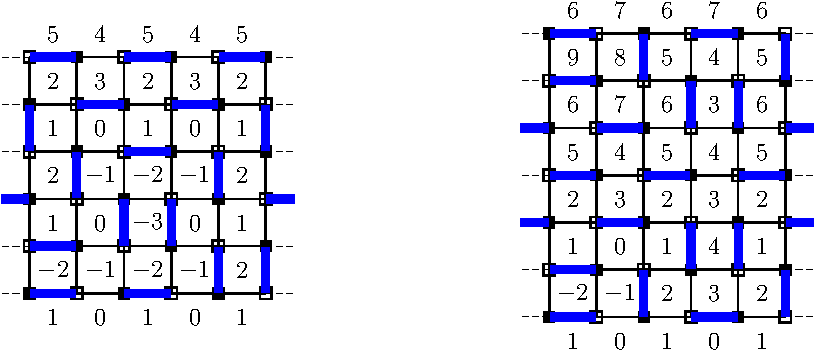
\includegraphics[scale=0.8]{./figures/shift.pdf}
 \end{center}
\caption{Illustration of the height shift between the upper and lower boundaries in the odd case.  \emph{Left:} Even $L_y$ case. The coarse-grained heigth difference between top and bottom is $\Delta h=\langle h_{\rm top}\rangle-\langle h_{\rm bottom}\rangle=(\pi/2)(9/2-1/2)=2\pi$.  \emph{Right:} Odd $L_y$ case. We have $\Delta h=(\pi/2)(13/2-1/2)=3\pi$.}
\label{fig:height_shift}
\end{figure}
These integers are defined by the following construction. Set value on one face (say the lower leftmost one) to be zero. Then, turning counterclockwise around a site of the even (resp.\ odd) sublattice represented by black squares (resp.\ white squares) the integer changes by $-3$ (resp.\ $+3$) if it crosses a dimer, $+1$ (resp.\ $-1$) otherwise. Since by construction these integers are different on adjacent sites, in the bulk one defines a smoother height variable $h(i,j)$ on the sites of the lattice, by averaging the values of the integers on four faces surrounding each point (and then for convenience's sake multiplying by $\pi/2$). Then the states where the dimers are arranged in columns correspond to a constant value of the height.

An important subtlety in this mapping is the boundary conditions, which will play a crucial role in understanding the even/odd effect in the two-cylinder Renyi entropy.
With periodic boundary conditions and an even number of sites around this cycle (as in the left and right sides of the figure \ref{fig:height_shift}), note that means that heights can jump by $2\pi$ times an integer on from one side to the other. 
With open boundary conditions, as we have at the ends of the cylinder (the top and bottom of the figure), the natural definition of the boundary height comes from averaging the integers along the boundary. For a cylinder of even $L_x$ circumference and length $L_y$, it is easy to check that the height difference between top and bottom satisfies \cite{Ferdinand}
\begin{equation}
 \Delta h=h(x,L_y)-h(x,0)=\left\{
 \begin{array}{ccc}
  2\pi w \quad,\quad w\in \mathbb{Z}&&L_y \;\;{\rm even}\\
  2\pi (w+1/2) \quad,\quad w\in \mathbb{Z}&&L_y \;\;{\rm odd}
 \end{array}
 \right.
\end{equation}
Even/odd effects have long been studied in the dimer model \cite{Ferdinand,Dimers_all,Ruelledimers}, but to our knowledge they have never been interpreted in the context of the height mapping. 

 
The standard Coulomb-gas arguments \cite{Nienhuis} then imply upon coarse-graining the height variable $h(i,j)$ into a continuous field, the scaling limit of the classical dimer model is described by a free scalar field $h(x,y)$ with euclidean action
 \begin{equation}\label{eq:free_field_bis}
  S_\kappa[h]=\frac{\kappa}{4\pi}\int \left(\nabla h\right)^2 dx dy\ .
 \end{equation}
The coupling $\kappa$ is often known as the ``stiffness''; we show below that for the dimer case it is set to $\kappa_D=1/2$. This free-boson field theory is one of the simplest examples of a two-dimensional conformal field theory \cite{Ginsparg}. It is ubiquitous in two-dimensional statistical models, as well as in condensed matter, where it describes Luttinger liquids.  In order to be consistent with periodic boundary conditions, field values shifted by $2\pi$ must be identified; in conventional language it is said that the field $h$ is compactified on a circle of radius $1$: $h\sim h+2\pi$. 

The dimers are viewed as elementary electric charges, i.e.\ are created by the field $\cos(h)$ (note that this is the simplest function of $h$ that satisfies the compactification $h\sim h+2\pi$). The standard computation \cite{Nienhuis} gives for the dimer-dimer correlator decay exponent:
\begin{equation}
 \alpha=\frac{1}{\kappa}\ .
\end{equation}
This yields the stiffness for the dimer model $\kappa_D=1/2$. Elementary magnetic charges can also identified with monomers, and the corresponding exponent describing their two-point function is given by $\beta=\kappa$, so $\beta_D=1/2$.
Once the stiffness fixed to its right value, Eq.~(\ref{eq:free_field_bis}) describes all the universal properties of the classical dimer model. By virtue of the correspondence between correlators in the classical model and those in the dimer RVB state, the same exponents apply to the correlators in the latter as well. 

In this framework the quantum dimer and quantum six vertex models can also be written as in terms of a free scalar field in the 2+1 dimensional ``quantum Lifshitz'' model \cite{Henley}. This is a field theory version of an RK Hamiltonian \cite{QuantumLifshitz}, and so where the equal-time correlators of a 2d {\em quantum} model are those of a 2d conformal field theory. This model is critical but not Lorentz-invariant, with dynamical critical exponent $z=2$.

Because of the arguments above, it is reasonable to hope that all the equal-time correlators in the $SU(N)$ RVB state for any $N$ can be described by this Coulomb gas, albeit with stiffness depending on $N$. Substantial evidence for this was provided in the $SU(2)$ case in \cite{RVB2}, where several universal quantities, including the dimer-dimer and monomer-monomer decay exponents, were found numerically. With appropriate identification of the operators, each yields a independent value for the stiffness.  The numerics gave approximately the same value of the stiffness $\kappa_{2}\approx .83$ for each, providing strong evidence that the Coulomb gas description applies to correlators of {\em spin singlets} in the $SU(2)$ RVB wave function. 

%\subsection{The RVB and Coulomb gas states}
%\label{sec:cg}

%This wavefunction can also be written as a superposition of classical ``loop'' states, defined by the transition graph formed by superimposing one element of the sum over $\alpha$ with some reference state.\footnote{\textcolor{blue}{This can be seen by computing the norm $\langle \Psi|\Psi\rangle=\sum_{{\rm loops}}2^{{\cal N}+2{\cal L}}$, where the sum runs over all the possible loop configurations. ${\cal N}$ is the number of double-edges and ${\cal L}$ is the number of non trivial loops.}}
%Correlators in the RVB can be written in terms of the correlators of this 2D classical loop model, where loops longer than length two have a weight of $4$ per loop (\textcolor{red}{THE DEFINITION OF ``WEIGHT'' NEEDS EXPLAINING}). A spin-spin correlator corresponds to having a strand of loop end at the sites of the spins \cite{LDA}. Such a correlator is exponentially decaying  whenever the weight per loop is greater than 2 \cite{Nienhuis}.  Moreover, extensive numerics indicate \cite{RVB1,RVB2} have not found any  spin order. 
%In this sense, the spins are ``deconfined'' and this state perhaps represents a sort of spin liquid.




\section{Two-cylinder Renyi entropy from partition functions}
\label{sec:shape_general}
%\subsection{Statement of the result}
In this section, we discuss the shape-dependent subleading contribution to the entanglement entropy 
of two-dimensional gapless systems discussed in \cite{Ju2012}. For Renyi index $n$ larger than a certain critical value $n_c$, we derive it exactly for the scaling limit of the square-lattice dimer RVB state, the quantum six-vertex state, and the entire quantum critical line of the quantum Lifshitz theory. Thus we expect it to apply to the scaling limit of the $SU(N)$ RVB state as well, with an appropriate parametrization of $\kappa$ in terms of $N$.

In particular, we show that when a  torus is split into two cylinders labeled $A$ and $B$, the Renyi entropy describing the entanglement between the two cylinders can be rewritten in terms of conformal field theory partition functions ${\cal Z}$ as:
\begin{equation}\label{eq:shape_general}
 s_{n>n_c}=\frac{n}{1-n}\ln \left(\frac{{\cal Z}_{A}{\cal Z}_B}{{\cal Z}_{\rm torus}}\right),
\end{equation}
Below we detail the precise definition of the CFT partition functions, but the important fact is that for the cases at hand, these are known. Thus this expression gives an explicit formula for this entropy, exact in the scaling limit. The value of $n_c$ depends on the specifics of the model, but $n_c<2$ in all the examples we will consider, so that Eq.~(\ref{eq:shape_general}) applies to the second Renyi entropy to be studied numerically in later sections.  Although our derivation applies only to the quantum Lifshitz ground state (i.e.\ RVB-type states that can be written in terms of a two-dimensional classical free boson), we believe it possible that an analogous formula will apply to any theory with an RK-type Hamiltonian.


\subsection{Entanglement entropy as a Shannon entropy}
\label{sec:eeshannon}

We will now detail how to derive Eq.~(\ref{eq:shape_general}), in the simplest case of quantum dimers on the square lattice. This requires a slight generalization of two ingredients: the mapping to a classical Shannon entropy of Ref.~\cite{Shannonee} (see Sec.~\ref{sec:eeshannon}) and the boundary phase transition argument of Ref.~\cite{Stephan2011} (see Sec.~\ref{sec:bpt}). Although this derivation does not apply to the $SU(N)$ RVB case, we will later explain why we think Eq.~(\ref{eq:shape_general}) should still apply.

The orthogonality of the different dimer configurations in the dimer RVB state allows for huge technical simplifications. As was shown in Ref.~\cite{Shannonee}, the entanglement entropy can be expressed as a classical Shannon entropy. We give here only a brief summary of the results, and refer to \cite{Shannonee} for the details.

Let us cut our torus in two subsystems $A$ and $B$, as is shown for example in Fig.~\ref{fig:bipartition}. We label the dimer configurations along the boundaries as $|\sigma\rangle$ and $|\mu\rangle$.
\begin{figure}[ht]
\begin{center}
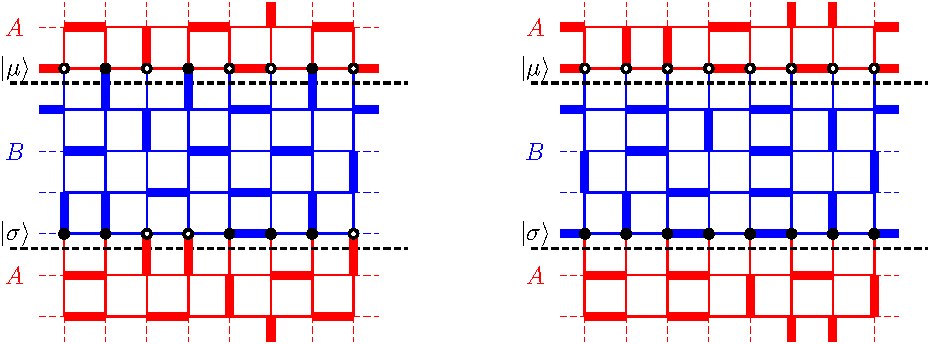
\includegraphics[scale=0.8]{./figures/bipartition.pdf}
\end{center}
\caption{Bipartition of the $8\times 8$ torus. The two boundaries between $A$ and $B$ are emphasized by thick dashed lines. Links crossing the lower boundary are defined to be in $A$, whereas those crossing the upper boundary in $B$.}
\label{fig:bipartition}
\end{figure}
The main difference with \cite{Shannonee} is that there are two boundaries here, but the the same arguments apply. The von Neumann entropy can be recast as a classical Shannon entropy
\begin{equation}
 S=-\sum_{\sigma,\mu} p_{\sigma,\mu} \ln p_{\sigma,\mu}
\end{equation}
where the $p_{\sigma,\mu}$ are the probabilities of a given boundary configuration $|\sigma\rangle$,$|\mu\rangle$ between $A$ and $B$. 
\label{sec:lg.}
The $\psm$ are precisely the eigenvalues of the reduced density matrix. Said differently, the Schmidt decomposition of the ground state reads
\begin{equation}\label{eq:schmidt}
|\psi\rangle=\sum_{
\sigma,\mu} \sqrt{p_{\sigma,\mu}}|\psi_{\sigma,\mu}^A\rangle |\psi_{\sigma,\mu}^B\rangle,
\end{equation}
where $|\psi_{\sigma,\mu}^A\rangle$ is a superposition of all dimer states in $A$ compatible with the boundary conditions $\sigma$ and $\mu$, and the same goes for $B$. All these vectors are mutually orthogonal
\begin{equation}\label{eq:schmidt_orthogonality}
\langle \psi_{\sigma,\mu}^\Omega|\psi_{\sigma^\prime,\mu^\prime}^{\Omega^\prime}\rangle=\delta_{\sigma \sigma^\prime}\delta_{\mu \mu^\prime}\delta_{\Omega \Omega^\prime},
\end{equation}
as should be. This mapping therefore allows the R\'enyi entanglement entropy to be rewritten as
\begin{equation}
 S_n=\frac{1}{1-n}\ln \left(\sum_{\sigma,\mu}[\psm]^n\right).
 \label{Spsm}
\end{equation}
We will name this quantity R\'enyi-Shannon entropy in the following. Note that here $n$ need not be an integer. The probabilities can be conveniently rewritten in terms of dimer partition functions as 
\begin{equation}
 \psm=\frac{Z_{\sigma,\mu}}{Z},
 \label{Zpsm}
\end{equation}
where $Z_{\sigma,\mu}$ is the number of dimer configurations compatible with the boundary configuration $|\sigma\rangle,|\mu\rangle$, while $Z$ is the number of dimer coverings on the whole torus. 

At this stage it is important to emphasize the main reasons why such a remarquable quantum-classical correspondance actually holds. While (\ref{eq:schmidt}) remains true for all the states we consider in this paper, the orthogonality (\ref{eq:schmidt_orthogonality}) is guarantied only if two other conditions are satisfied:
\begin{enumerate}
 \item The orthogonality of quantum states corresponding to different classical configurations. 
 \item A certain type of local constraints\cite{Shannonee}, which one can summarize as follows on the square lattice. Formulating the model as Ising variables $\sigma$ sitting on the bonds of the square lattice (for dimers these are just the dimer occupancies) the following constraint is needed: around each site of the lattice, if three of them are specified, then the state of the last one is uniquely determined.  
\end{enumerate}
Quantum dimers obviously satisfy both these requirements. The same goes for the quantum six-vertex state, (ii) being guarantied by the ice rule. The $SU(N)$ RVB wave functions satisfies (ii) but not (i) (see (\ref{eq:nonortho})). As an example of Coulomb-gas wave functions that satisfy (i) but not (ii), one can consider the quantum dimer wave function built out of the interacting dimer studied in \cite{Alet_dimers1,Alet_dimers2}. 

Returning to the dimer RVB state, these expressions make it possible to use the computer to find very accurate values for the Renyi entropy. Using free-fermion/Pfaffian techniques described in \ref{sec:lgv}, each probability can be expressed as a product of determinants of two matrices of size $\sim L/2$, and computed numerically in a time of order $\approx L^3$. Using translational symmetry along the $x$ axis as well as the conservation of winding numbers, we are able to compute any R\'enyi entropy up to machine precision in a time of order $L^{3/2}\times 4^L$.
The results for a $20\times 20$ torus are summarized in Fig.~\ref{fig:ee_d_torus}, where the two cylinders are of length $\ell_y$ and $L_y-\ell_y$. 
\begin{figure}[ht]
 \begin{center}
 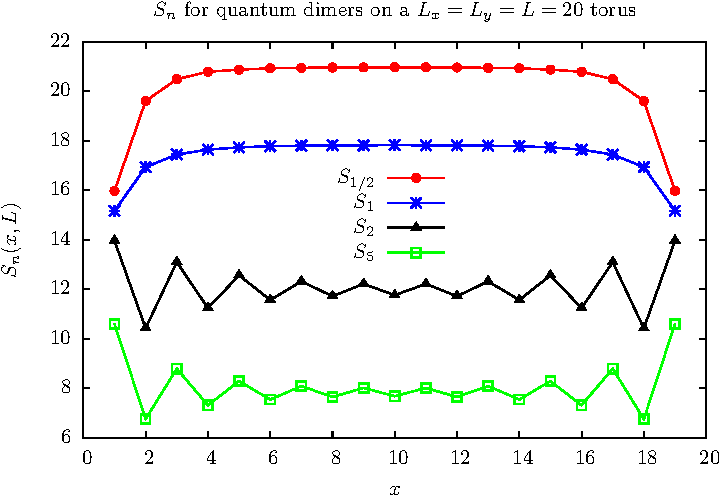
\includegraphics[width=10cm]{./figures/ee_d_torus.pdf}
 \end{center}
\caption{Two-cylinder R\'enyi entanglement entropies $S_{1/2}$, $S_1$, $S_2$ and $S_5$ for the dimer RVB state on the square lattice in the torus geometry. Here $L_x=L_y=20$.}
\label{fig:ee_d_torus}
\end{figure}
The figure makes it obvious that the Reyni entropy exhibits strikingly different behavior for different values of $n$. In the ``replica'' phase $n \leq 1$, the curves are relatively flat. In the thermodynamic limit we expect them to go to universal functions, which in principle may be computed within boundary CFT, although we will not study this phase here. For $n$ large enough, we observe a striking even-odd effect like that observed for the $SU(2)$ RVB state in \cite{Ju2012}. We explain the origin of this transition in dimer RVB state in the next subsection.



\subsection{The entropy in the locked phase $n>n_c$}
\label{sec:bpt}
Here we derive the relation of the two-cylinder entanglement entropy of the dimer RVB state to CFT partition functions in 
(\ref{eq:shape_general}) for $n>n_c$. This follows fairly simply from the description of the long-distance behavior of classical dimers in terms of the free boson action (\ref{eq:free_field_bis}).

When one utilizes an effective field-theory action to describe the scaling limit of a lattice model, one must include all terms in the action consistent with the symmetries of the field theory. As is familiar from the derivation of the Kosterlitz-Thouless transition in field theory, operators of the form 
\begin{equation}
 V_d=-\cos \left(d \,(h-h_0)\right)
 \label{Vdef}
\end{equation}
with $d$ integer 
are consistent with the compactification  of the boson $h\to h + 2\pi$.
If such a term is relevant, then the action flows to a configuration where the height $h$ is locked to one if the minimal values $h=h_0$ mod $2\pi$. For dimers on the square lattice, it has long been known that any such term allowed are irrelevant in the bulk; this is why the action (\ref{eq:free_field_bis}) applies and the correlators are algebraically decaying. However, we showed in the preceding subsection \ref{sec:eeshannon} that the probabilities used to compute the Renyi entropy depend on the boundary conditions. Thus the crucial observation of \cite{Stephan2011} (see also \cite{Shannonee}) is that one needs to include terms of the form (\ref{Vdef}) localized at the {\em boundary}.

To be precise, in the continuum limit the probabilities $p_{\sigma,\mu}$ depend now on the configurations of the field $p(\phi)$. The probability of observing field configuration $\phi$ at the boundary is still gaussian
\begin{equation}
 p(\phi)\propto \exp(-S_{\kappa}[\phi]),
\end{equation}
and raising this probability to the $n-$th power yields
\begin{equation}
 [p(\phi)]^n=\exp(-n S_{\kappa}[\phi])=\exp(-S_{n\kappa}[\phi]).
\end{equation}
Therefore, the system near the boundary effectively feels a stiffness $\kappa^\prime=n\kappa$. 
Standard Coulomb gas/field theory then computations (see e.g.\ \cite{Nienhuis}) give the boundary scaling dimension of (\ref{Vdef}) to be $d^2/(2n\kappa)$. 
As a consequence, $V_d$ is irrelevant as long as $d^2>2n\kappa$. Thinking of $n$ as a continuous parameter, this defines two regions, separated by a (boundary) Kosterlitz-Thouless phase transition. The critical value of $n$ in the computation of  $S_n$  is therefore
\begin{equation}
 n_c=\frac{d_{\rm min}^2}{2\kappa},
\end{equation}
where $d_{\min}$ is the smallest $d$ allowed by the lattice symmetries. For dimers on the square lattice $d_{\rm min}=1$ and $\kappa=1/2$, so that the critical value is
\begin{equation}
 n_c=1.
\end{equation}
The two qualitatively different types of behavior seen in fig.\ \ref{fig:ee_d_torus} indeed occur on opposite sides of $n_c$. It is important to note that even though $S_n$ should take an universal form in both phases, the value itself of the critical R\'enyi parameter depends on a degeneracy $d_{\rm min}$, which is non-universal. For example, $d_{\rm min}=2$ for the quantum six-vertex wave function, and $d_{\rm min}=3$ for quantum dimers on the hexagonal lattice. 

This observation allows us to derive the expression for $S_n$ valid for $n>n_c$. In this phase, the boundary operator is relevant. This means that here the boundary value of the field locks on to a minimum of $V_1$. This minimum must be fixed along the entire boundary; this is commonly known as Dirichlet boundary conditions on the boson. We refer therefore to the phase with $n>n_c$ as the ``locked'' phase.

A constant value of the field along the boundary means that the action is at its minimum there, so this is the {\em maximum} value of the probability $p_{\rm max}$. 
Universal contributions to the R\'enyi entropy coming from the sum (\ref{Spsm})  are therefore dominated by the configuration:
\begin{equation}\label{eq:aftert}
 S_{n>n_c}\sim \frac{n}{1-n}\ln (p_{\rm max})
\end{equation}
This result implies that in the scaling limit there is an ``entanglement gap'' between $p_{max}$ and the other values. We have confirmed directly the presence of the entanglement gap for the dimer RVB state by numerical evaluation of the probabilities using the free-fermion techniques detailed in \ref{sec:lgv}.  This is distinct from the quantum Hall case \cite{HaldaneLi}, where there is no entanglement gap, in correspondence with the gapless edge excitations there.
 
 In terms of dimers, the configuration with maximum probability corresponds to no dimers crossing the boundaries between $A$ and $B$ (see Fig.~\ref{fig:bipartition}). This is a huge technical simplification, since the probability of having no dimers across the cut factorizes into pieces coming from region $A$ and from region $B$. Namely, define $Z_{\rm cyl}(L_x, L_y)$ to be the partition function (the number of dimer configurations) for a cylindrical region of size $L_x$ in the periodic direction and $L_y$ in the other, with boundary conditions corresponding to no dimers leaving the region. Likewise, $Z_{\rm torus}(L_x,L_y)$  is the number of dimer configurations with periodic boundary conditions. Then it follows from (\ref{Zpsm}) that when an $L_x\times L_y$ torus is split into cylinders of lengths $\ell_y$ and $L_y-\ell_y$,
\begin{equation}\label{eq:pmax}
 p_{\rm max}=\frac{Z_{\rm cyl}(L_x,\ell_y)Z_{\rm cyl}(L_x,L_y-\ell_y)}{Z_{\rm torus}(L_x,L_y)} \ .
\end{equation}
The analogous formula still holds if space is a cylinder instead of a a torus, simply by replacing the denominator with the appropriate cylinder partition function. Note that the non-universal bulk parts of the partition functions cancel in this expression, so that one can use the universal partition functions computed in the free-boson conformal field theory. Thus putting (\ref{eq:pmax}) together with (\ref{eq:aftert}) gives (\ref{eq:shape_general}). 


For the dimer RVB state, the partition functions on the cylinder can be computed exactly both on the lattice and in the continuum.  The lattice dimer result is detailed in \ref{sec:dimers_exact}. For the free-boson field theory, these partition functions are known explicitly \cite{BigYellowBook};  we will discuss their application to the two-cylinder Renyi entropy in the next section \ref{sec:dimers_entanglement}. In particular, we will show how the even-odd effect is a signature of this locked phase  $n>n_c$, arising from the different boundary conditions necessary for the even and odd sectors.


It should also be possible to extend these results to the region $n<n_c$, using boundary CFT methods \cite{Shannonee,Oshikawa,Zaletel,Stephan2011}. Here, however, the boundary conditions will presumably not allow the factorization of the probability into pieces coming from the two regions. Oshikawa\cite{Oshikawa} has already treated the $y=1/2$ case for the closely related cylinder geometry, using the replica approach $n\in \mathbb{N}$. There will possibly be subtleties involving analytic continuation in $n$, similar to the two-interval 1d calculation \cite{CCT1,CCT2}.


\section{Entanglement in the dimer RVB state}
\label{sec:dimers_entanglement}

This section is devoted to the exploration of the consequences of Eq.~(\ref{eq:shape_general}) for the two-cylinder Renyi entropy of the dimer RVB state. We will calculate explicitly the partition functions, and so find results exact in the scaling limit. 

The main subtlety in this computation is how to account in the field theory for the distinct results occurring when the cylinders are of even and of odd length, as apparent in the numerical results in fig.\ \ref{fig:ee_d_torus} for the dimer RVB state and those in \cite{Ju2012} for the $SU(2)$ RVB state. The reason this is possible in the field theory is that a fixed/Dirichlet boundary condition is in fact a family of boundary conditions, corresponding to the specific value $h_0$ that the field takes at a boundary. This value can be always be shifted overall, since the bulk action used to compute the partition functions is independent of it. However, on a cylinder, there are two separate boundaries, and what cannot be shifted away is the {\em difference} of the values on the two ends.    
The general arguments given above in section (\ref{sec:bpt}) do not specify this difference; it follows rather from the particular microscopic model. For dimers, we showed in section \ref{sec:cg} that 
\begin{equation}
 \Delta h =2\pi (w+a)\quad,\quad w \in \mathbb{Z},
\end{equation}
where $a=0$ for even $L_y$ and $a=1/2$ for odd $L_y$. 


The computation of the free-boson partition function is completely standard; see e.g.\ \cite{EggertAffleck,FSW,BigYellowBook}. Since the action is quadratic in the bosonic field, it can be decoupled into an oscillator part and a classical part. Only the classical part affected by the compactification $h\sim h+2\pi$, and by the boundary conditions. The partition function for Dirichlet boundary conditions on both ends of the cylinder, with the height differing by $a$, is given by
%\begin{equation} \mathcal{Z}_{\rm cyl}^{DD^{(a)}}=e^{\frac{\pi}{24}\frac{L_x}{L_y}}\prod_{w=1}^{\infty}\left(1-e^{-\pi w\frac{L_x}
%{L_y}}\right)^{-1}\sum_{w=-\infty}^{+\infty}e^{-\kappa \pi\frac{L_x}{L_y} (w+a)^2}.
%\end{equation}
\begin{equation}
 \mathcal{Z}_{\rm cyl}^{DD^{(a)}}=q^{-1/24}\prod_{w=1}^{\infty}\left(1-q^w\right)^{-1}\sum_{w=-\infty}^{+\infty}q^{\,\kappa (w+a)^2}\quad,\quad q=e^{-\pi L_x/L_y}
\end{equation}
It is convenient to rewrite such sums in terms of the Jacobi theta and Dedekind eta functions defined in \ref{sec:CFT_Jacobi}, to take advantage of many elegant identities. 
The even case $a=0$ can be written, using (\ref{eq:eta_def},\ref{eq:theta3_def},\ref{eq:thetas},\ref{eq:modtheta3},\ref{eq:modeta}), as
\begin{equation}\label{eq:cylinder_dd}
 \mathcal{Z}_{\rm cyl}^{DD}(\tau)=\frac{\theta_3(2\tau)}{\eta(2\tau)}\ ,
\end{equation}
where we adopt the conventional variable  $\tau=i L_y/L_x$, and have set $\kappa=1/2$, the dimer value.
For the odd case $a=1/2$, we have, using this time (\ref{eq:eta_def},\ref{eq:theta2_def},\ref{eq:thetas},\ref{eq:modtheta4},\ref{eq:modeta}):
\begin{equation}
\label{eq:cylinder_ddprime}
 \mathcal{Z}_{\rm cyl}^{DD^\prime}(\tau)=\frac{\theta_4(2\tau)}{\eta(2\tau)}\ .
\end{equation}

Plugging these results into Eq.~(\ref{eq:shape_general}) and using the torus partition function\cite{Ginsparg,BigYellowBook} gives for the two-cylinder entanglement entropies
\begin{eqnarray}\label{eq:cft_prediction}
 s_n^{\rm (even)}(y,\tau)&=&\frac{n}{1-n}\ln \left(\frac{\eta(\tau)^2}{\theta_3(2\tau)\theta_3(\tau/2)}\times\frac{\theta_3(2y \tau)\theta_3(2(1-y)\tau)}{\eta(2y\tau)\eta(2(1-y)\tau)}\right)\ ;\\
 \label{eq:cft_prediction_odd}
 s_n^{\rm (odd)}(y,\tau)&=&\frac{n}{1-n}\ln \left(\frac{\eta(\tau)^2}{\theta_3(2\tau)\theta_3(\tau/2)}\times\frac{\theta_4(2y \tau)\theta_4(2(1-y)\tau)}{\eta(2y\tau)\eta(2(1-y)\tau)}\right)\ .
\end{eqnarray}
Fig.~\ref{fig:dimers_shape} shows a numerical test of the universal shape Eq.~(\ref{eq:cft_prediction}) for the dimer RVB states with two different aspect ratios $L_y/L_x=1$ and $L_y/L_x=2$.  
\begin{figure}[ht]
\begin{center}
 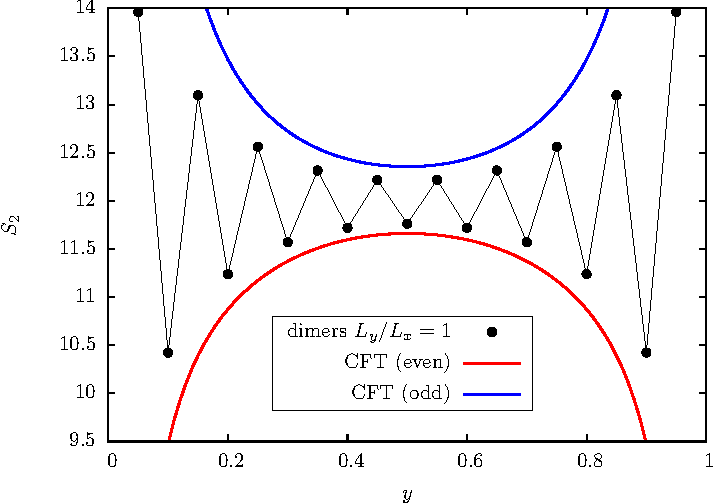
\includegraphics[width=8cm]{./figures/dimers_shape.pdf}
 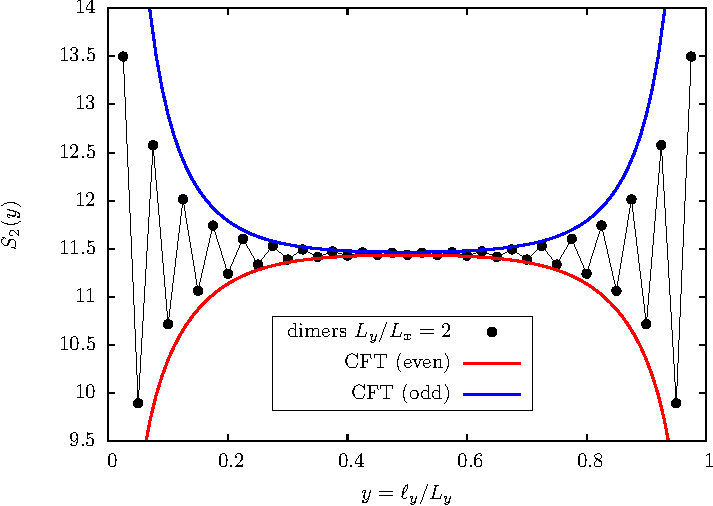
\includegraphics[width=8cm]{./figures/dimers_shape2.pdf}
 \end{center}
 \caption{Numerical results for the second R\'enyi entropy $S_2$ as a function of the subsystem-ratio $y=\ell_y/L_y$ for $L_x=20$. Black dots are the data for square-lattice dimer RVB state, while the CFT predictions are given by Eq.~(\ref{eq:cft_prediction}) in the even case and Eq.~(\ref{eq:cft_prediction_odd}) in the odd case. \emph{Left:} Torus with aspect ratio $L_y/L_x=1$. \emph{Right:} Torus with aspect ratio $L_y/L_x=2$.}
 \label{fig:dimers_shape}
\end{figure}
Obviously, these $n>n_c$ results are quite different in the even and odd sectors. The difference is proportional to $n/(n-1)$, and therefore slightly diminishes with increasing $n$, but does not go away. 


This even/odd effect disappears as $L_y/L_x$ is increased; it follows from the CFT expressions that this occurs exponentially quickly.  It does not approach the celebrated 1d result\cite{Cardy} $\propto \ln\sin (\pi y)$ in the effective 1d limit $L_y/L_x\to\infty$, because the RK Hamiltonian becomes gapped with correlation length $\xi\propto L_x$ in this limit. 

%It could have been tempting to expect the result to be similar to the celebrated 1d quantum result$S_n\propto \ln\sin (\pi y)$ in the infinite torus limit. This is clearly not the case, and one can easily check that the corresponding quasi-1d system would be gapped, and therefore cannot exhibit the conformal scaling. 


%The even-odd effect is much less pronouced in for larger $L_y/L_x$, compatible with our prediction that $S_2$ goes exponentially fast in $L_y/L_x$ to a single flat curve. 


The relatively large finite-size effects apparent in the plots should disappear in the thermodynamic limit.  To illustrate the slowness of the convergence, we study the exactly solvable case $S_\infty=-\ln p_{\rm max}$ (Eq.~(\ref{eq:pmax})), where the agreement between CFT and the lattice can be made rigorous. 
%$s_{\infty}$ is obtained by taking the $n\to \infty$ limit in Eq.~(\ref{eq:cft_prediction}). 
We also compute $s_\infty$ in the $W=(0,0)$ winding sector directly for the dimer model, using the techniques described in the appendices, finding:
\begin{eqnarray}\label{eq:cft_w0}
 s_\infty^{\rm (even)}&=&-\ln \left(\frac{\eta(\tau)^2\theta_3(2y(1-y)\tau)}{\eta(2y\tau)\eta(2(1-y)\tau)}\right)\\\label{eq:cft_w0_odd}
 s_\infty^{\rm (odd)}&=&-\ln \left(\frac{\eta(2\tau)^2\theta_4(2y(1-y)\tau)}{\eta(2y\tau)\eta(2(1-y)\tau)}\right)
\end{eqnarray}
Even though the total winding number is zero, the result still depends on the compactification radius of the height field  because of winding fluctuations at the boundaries between regions $A$ and $B$. 
A comparison between the numerical and analytical results is performed in Fig.~\ref{fig:Sinfty}, for the aspect ratio $L_y/L_x=1$ and the two system sizes $L_x=16$ and $L_x=704$. We observe strong finite-size effects for small system sizes, but the data converges in the end to the CFT result.
\begin{figure}[ht]
 \begin{center}
  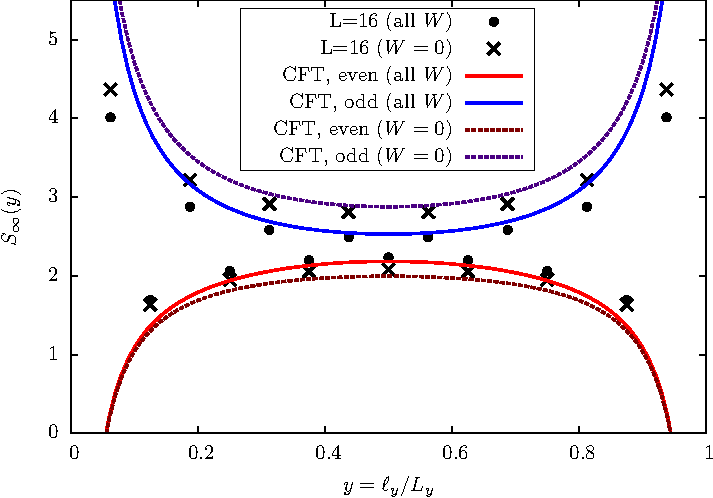
\includegraphics[width=8cm]{./figures/sinfty_16.pdf}
  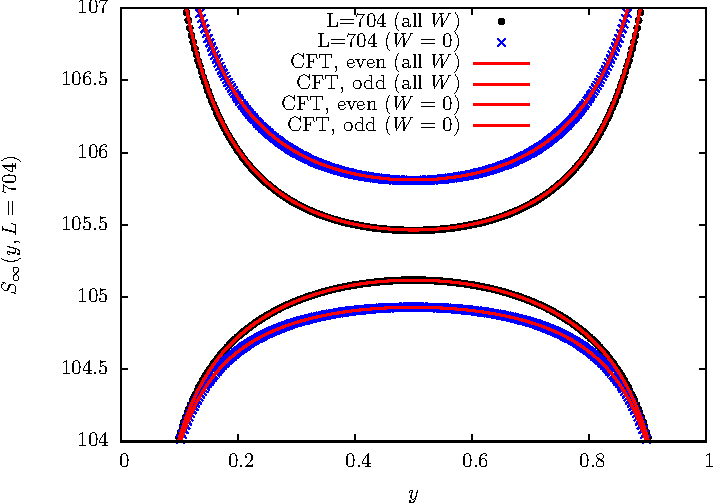
\includegraphics[width=8cm]{./figures/sinfty_704.pdf}
 \end{center}
\caption{Comparison numerics/analytics in the exactly solvable case $S_\infty$. Black points are the numerical data for all winding sectors, and black crosses represents the numerical data in the $W=(0,0)$ sector. \emph{Left:} $L_x=16$, the data is compared with Eqs.~(\ref{eq:cft_prediction}), (\ref{eq:cft_prediction_odd}),  (\ref{eq:cft_w0}) and (\ref{eq:cft_w0_odd}) up to a single constant. The agreement is fair, but still far from converged. \emph{Right:} Same procedure for $L=704$. The agreement is close to perfect, as expected. }
\label{fig:Sinfty}
\end{figure}

%\begin{equation}\label{eq:shape_general2}
% s_{n>n_c}=\frac{n}{1-n}\ln \left(\frac{{\cal Z}_{\rm cyl}[y\tau]{\cal Z}_{\rm cyl}[(1-y)\tau]}{{\cal Z}_{\rm torus}[\tau]}\right),
%\end{equation}

%  \item Since the problem has been reduced to a ratio of partition function, this result is different from the 1d critical case\cite{Cardy} $S\propto \ln \left|(L/\pi)\sin (\pi y/L)\right|$. Therefore, eventhough the 1d result can provide interesting physical intuition, it \emph{should not} apply in higher dimensions. This had already been noted in \cite{Ju2012} wave functions with different dynamical exponents: $\pi$-flux fermions on the square lattice.  




\section{Correlations in the $SU(N)$ RVB wave function}
\label{sec:correlations}
We now start to explore the question of universality, with the motivation of understanding whether the results obtained for the dimer RVB state can be adapted to apply to the $SU(N)$ RVB states. In this section we describe the use quantum Monte Carlo techniques to find the spin-spin and dimer-dimer correlators for $N=2,3,4,5$, generalizing some of the results of \cite{RVB1,RVB2}. This shows that there is no evidence for a transition as $N$ is varied, a strong piece of evidence for universality. It also allows us to make contact with the results of \cite{Damle}, where an expansion around the dimer RVB state is developed.

%$SU(N)$-RVB wave function, before going to its entanglement properties (Sec.~\ref{sec:rvb_entanglement}). This section, which may be skipped at first reading, is organized as follows. In Sec.~\ref{sec:numerics}, we explain how such systems , in particular their correlation functions, maybe be simulated using Quantum Monte Carlo techniques. We then study spin-spin correlations, as well as the more interesting dimer-dimer correlations. We find that dimer-dimer correlations decay algebraically, and that the exponent interpolates between $SU(2)$\cite{RVB1,RVB2} and the pure dimer exponent ($N\to \infty$), in agreement with a recent large $N$ calculation\cite{Damle}.

\subsection{Numerical methods}
\label{sec:numerics}

To study $SU(N)$-RVB wavefunctions, we use an unbiased Monte Carlo technique that calculates expectation values in the equal-amplitude superposition of states using an importance sampling scheme in the valence-bond (VB) basis.  Like employed previously for the $SU(2)$ case \cite{Ju2012}, one must use a non-local
loop updating scheme in order to efficiently (and ergodically) sample all possible RVB states \cite{sandvik2010loop}.
This loop update moves through the ensemble of states by creating a defect at some lattice site and propagating it through the system until the defect reaches its initial point, thus closing the loop.  Unlike the $SU(2)$ updates used in Ref.~\cite{RVB2}, one must generalize such loop updates to account for $SU(N)$ RVB wavefunctions.  To do so, one first forms the transition graphs to compute Eq.~(\ref{eq:overlap}) at every Monte Carlo step. Using this transition graph, one samples the value of $m \equiv S^z$ at each site. This gives a larger set of constraints in that the loop can only update within a compatible $m$ as defined in Eq.~(\ref{eq:rvb}). Then, the case of $N=2$ is equivalent to having two independent subsets; configurations can only be updated by loops that move within each subset. For a larger $N$, the number of updates that one can successfully make becomes much smaller, making the error bars much slower to converge.
%This can be cured by using a smarter update that satisfies detailed balance to allow the simulation to make more updates.
As described below, for $N \ge 4$ some estimators show signs of ergodicity loss; this might be cured by a more sophisticated sampling scheme in the future.

In our VB basis Monte Carlo simulations, we begin by computing the spin-spin and the dimer-dimer correlations. The expectation values were first derived in~\cite{beach2006some} and generalized in~\cite{beach2009n} for $SU(N)$ spins.  Using the notation $(ij)_L$ for two sites $i,j$ in the same loop in the transition graph and $(i)_L(j)_L$ for sites not in the same loop~\cite{RVB2},
\[ 
\displaystyle
\frac{\langle V_\mathcal{C} | \mathbf{S}_i \cdot \mathbf{S}_j | V_{\mathcal{C}'} \rangle}{\langle V_\mathcal{C} | V_{\mathcal{C}'} \rangle} = \left\{ \begin{array}{ccc}
0 & (i)_L (j)_L\\
\epsilon_{ij} \, S (S+1) & (ij)_L   \end{array}. \right.
\] 
Here, $\epsilon_{ij} = 1$ if $(i,j)$ are on the same sublattice and $\epsilon_{ij} = -1$ if they are on different sublattices.
We also measure \textit{parallel} nearest neighbor dimer-dimer correlations, i.e.
\[ 
\displaystyle
\frac{\langle V_\mathcal{C} | \left( \mathbf{S}_i \cdot \mathbf{S}_j \right) \left( \mathbf{S}_k \cdot \mathbf{S}_l  \right) | V_{\mathcal{C}'} \rangle}{\langle V_\mathcal{C} | V_{\mathcal{C}'} \rangle} = \left\{ \begin{array}{ccc}
\frac{1}{3} S^2 (S+1)^2 & (ik)_L (jl)_L, \,(il)_L (jk)_L\\
S^2 (S+1)^2 & (ij)_L (kl)_L \end{array}, \right.
\] 
and $0$ otherwise. Because we are measuring parallel dimer-dimer correlations, we take $j = i + \hat{e}_\alpha, \, l = k + \hat{e}_\alpha$ and $k = i + \hat{e}_\beta$, where $\alpha,\beta = x, y, \, \alpha \neq \beta$.

\subsection{Equal-time correlators}
\label{sec:dimerdimer}


The connected dimer-dimer correlation function has been recently shown to decay algebraically in the $SU(2)$ case in Refs.~\cite{RVB1} and \cite{RVB2}:
\begin{equation}\label{eq:decay}
 C_{dd}(\vec{r}_1,\vec{r}_2)\sim \frac{1}{\left|\vec{r}_1-\vec{r}_2\right|^\alpha}
\end{equation}
at distances large compared to the lattice spacing, but small compared to the torus size $L=L_x=L_y$. Using several different methods, the exponent was found to be approximately $\alpha \simeq 1.2$, independent of the direction.
We extend some of these results, on the $SU(N)$ case, mainly focusing on the correlations for two parallel dimers in the direction ($\vec{r}_1-\vec{r}_2=\ell_x \vec{u}_x$). 
Our quantum Monte Carlo results are shown in Fig.~\ref{fig:corr_su2_dimers} for a $L\times L$ torus, with $L=64$. The data clearly indicate that the algebraic decay remains for $N=2,3,4,5$, with $\alpha$ increasing with $N$. 
Since $SU(N)$ dimer correlations reduce to pure dimer correlations in the limit $N\to\infty$, we know that
$
 \lim_{N \to \infty} \alpha_N=\alpha_{\rm D}=2,
$
 and our data is consistent with the smooth interpolation between $N=2$ and $\infty$. \begin{figure}[ht]
 \begin{center}
  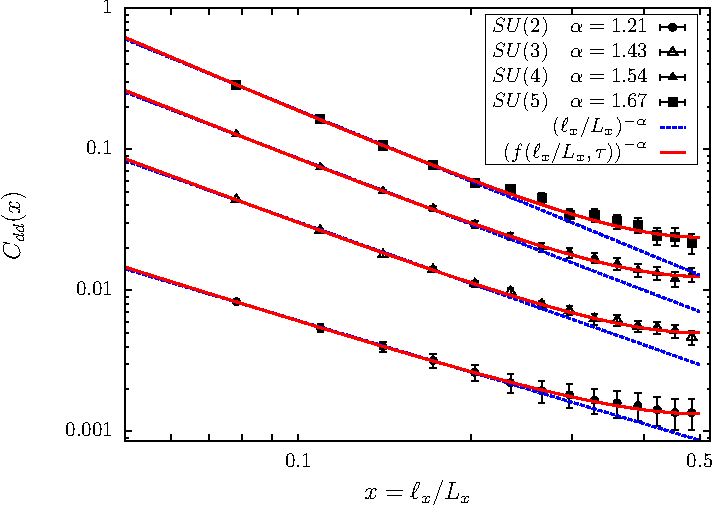
\includegraphics[scale=0.8]{./figures/corr_su2.pdf}
 \end{center}
\caption{Dimer-Dimer correlations on the $64 \times 64$ torus for $N=2,3,4,5$. Dashed blue lines is a linear fit to Eq.~(\ref{eq:decay}), in the ``linear regime'' $\ell_x \simeq 5,\ldots,15$, while the red solid lines are a fit to the conformal scaling (Eq.~(\ref{eq:cft_fit})) in the same region.}
\label{fig:corr_su2_dimers}
\end{figure}
For each $N$ we extract the leading exponent by a fit (solid blue lines in Fig.~\ref{fig:corr_su2_dimers}) to Eq.~(\ref{eq:decay}) in the regime $1\ll \ell_x \ll L_x$ and for odd $\ell_x$. We find $\alpha_2=1.21(7)$, $\alpha_3=1.43(7)$, $\alpha_4=1.54(8)$, $\alpha_4=1.67(9)$. Notice that as $N$ gets larger, it becomes more and more difficult to converge the Monte-Carlo data in a finite time, resulting in a loss of precision on the corresponding exponent. 

We also observe the presence of a dipolar term which behaves as $(-1)^{\ell_x} \ell_x^{-2}$ for all $N$. It is well known in the dimer model\cite{Alet_dimers2}, and also appears for the $SU(2)$ RVB state\cite{RVB2}. In the dimer case, it exactly cancels the universal term (\ref{eq:decay}) at even distances, so that the dimer-dimer correlation now behaves as\cite{FisherStephenson} $\ell_x^{-4}$. In the $SU(N)$ RVB case the exponent $\alpha$ is different and this does not happen. The dipolar is then a subleading term, which introduces finite-size effect when trying to extract the exponent. For example we get $\alpha_2\simeq 1.14$ at even distances, which is slightly smaller than the established value on larger system sizes\cite{RVB1,RVB2} for $SU(2)$, and probably less raliable. 


These values are in good agreement with the expansion around the dimer RVB state developed in \cite{Damle}. This is a cluster expansion of the loop model, describing the non-trivial inner product in (\ref{eq:overlap}) perturbatively in $1/N$ in terms of a classical interacting dimer model. 
To first nontrivial order, this model is exactly the one studied in \,\cite{Alet_dimers1,Alet_dimers2}, and so the Monte Carlo results in fig.\ 28 of \cite{Alet_dimers2} can be utilized; in their notation $X_2=\alpha/2$ and $W=1+1/N$. This gives, in addition to the already reported $\alpha_2\simeq 1.22$, $\alpha_3 \simeq 1.4$, $\alpha_4 \simeq 1.52$, and $\alpha_5\simeq 1.6$. Our numerical results therefore confirm that the leading-order term in this expansion gives accurate results.


A presumably more accurate value for $\alpha$ can be found relaxing the constraint $\ell \ll L$, and fitting the data to the full curve predicted by conformal field theory, not just the straight-line segment. While the two-point function on a torus is not fixed uniquely by conformal invariance, the appropriate form is known for the free boson field theory for any $\kappa$ \cite{BigYellowBook}. Thus if we assume that the free-boson/Coulomb gas results still apply with a different $\kappa=1/\alpha$,  the $SU(2)$ dimer-dimer correlators are modified to 
\begin{equation}\label{eq:cft_fit}
 D_{||}(\ell_x)\sim f(\ell_x/L_x,\tau)^{-\alpha},
\end{equation}
with $\ell_x \gg 1$. $f$ is a universal function of the two dimensionless ratios $\ell_x/L_x$ and $\tau =i L_y/L_x$ and can be expressed in terms of a Jacobi theta function defined in \ref{sec:CFT_Jacobi}. We have 
\begin{equation}
 f(\ell_x/L_x,\tau)=\sum_{n=0}^{\infty}(-1)^n \sin \left[(2n+1)\pi \ell_x/L_x\right]e^{-\pi n(n+1)(L_y/L_x)}
\end{equation}
Notice that while this function reduces to $f(\ell_x/L_x,\tau)=\sin(\pi \ell_x/L_x)$ in the limit of a thin torus ($L_y/L_x \gg 1$), the latter is still an almost perfect approximation for $L_y/L_x=1$. Performing the fits to Eq.~(\ref{eq:cft_fit}) in the same region $1\ll \ell_x \ll L_x$ as before (red solid curve in Fig.~\ref{fig:corr_su2_dimers}), we observe that the data reproduces very well the CFT prediction, even the upturn when $\ell_x$ is of order $L_x$. This is additional evidence for the underlying height model. However, the exponents determined this way are slightly larger; for example we find $\alpha_2\simeq 1.26$ in the odd case, and $\alpha\simeq 1.18$ in the even case. This small discrepancy with the previous $SU(2)$ results\cite{RVB1,RVB2} could possibly be resolved studying larger systems.  

\begin{figure}[ht]
 \begin{center}
  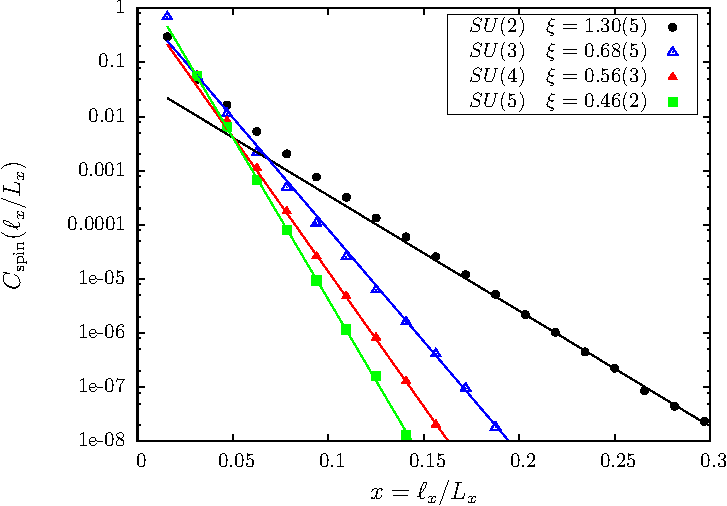
\includegraphics[scale=0.8]{./figures/spin_corr.pdf}
 \end{center}
\caption{Spin-spin correlation function on a $64\times 64$ torus. We look at spins separated by a distance $\ell_x$ along the $x-$ direction:  $\vec{r}_1-\vec{r}_2=\ell_x \vec{u}_x$. }
\label{fig:corrspin_su2}
\end{figure}
We also studied spin correlations, which as discussed in section \ref{sec:RVB} are known to decay exponentially in the $SU(2)$ case: 
$
 \langle S(0)S(\ell_x) \rangle \sim \exp \left(-{\ell_x}/{\xi}\right)
$
\cite{LDA,RVB1} .
We find the same behavior in the $SU(N)$ case, with our results displayed in Fig.~\ref{fig:corrspin_su2}. We also observe that $\xi$ decreases with $N$, compatible with the intuition that the RVB state becomes more and more spin-disordered as $N$ increases, approaching zero correlation length in the dimer limit $N\to\infty$. Fitting the data gives  $\xi(N=2)=1.30(5)$ (compatible with \cite{RVB1}) and $\xi(N=3)=0.68(5)$, $\xi(N=4)=0.56(3)$ and $\xi(N=5)=0.46(2)$. This lack of long-range N\'eel order is consistent with quantum spin-liquid  behavior. 




\section{Entanglement in the $SU(N)$ RVB wave function}
\label{sec:rvb_entanglement}

We finally turn to the entanglement in the $SU(N)$ RVB case, extending previous numerical results\cite{Ju2012} for $SU(2)$, and providing evidence that Eq.~(\ref{eq:shape_general}) still holds.

%\subsection{Numerical results for $SU(2)$}
%\label{sec:su2_numerics}
Let us first begin with the $SU(2)$ case, and present the computation of $S_2$, and also $S_2$ restricted to the $W=(0,0)$ winding sector. The quantum Monte Carlo data is shown in Fig.~\ref{fig:SU2_shape}.\begin{figure}[ht]
 \begin{center}
  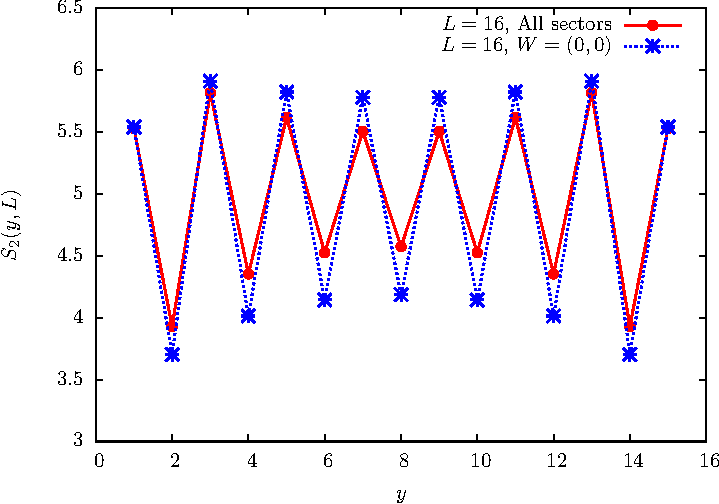
\includegraphics[width=10cm]{./figures/SU2_shape.pdf}
 \end{center}
\caption{Numerical extraction of the universal shape of $S_2$ as a function of $y=\ell_y/L_y$ for the $SU(2)$ RVB wave function and $L=L_x=L_y=12,18,24$. Red and blue curves are the CFT prediction of Eqs.~(\ref{eq:cft_prediction_gen}) and (\ref{eq:cft_prediction_gen_odd}). }
\label{fig:SU2_shape}
\end{figure}
We observe a striking similarity with the dimer data. In particular, the even-odd effect is bigger in the $W=(0,0)$ than in the ``all'' sector. >>> Should we provide a plot, maybe next to the other one???
This suggests $S_2$ for the $SU(2)$ RVB state lies in a locked phase, just as its dimer counterpart does. 
This is also supported by exact diagonalizations on small systems, which show that the biggest eigenvalue of the reduced density matrix is non-degenerate:  $\Delta_{SU(2)}\equiv -\ln (p_1/p_{\rm max}) \approx 2.67$ for on a $4\times 4$ torus. (The exact value for dimers is  $\Delta_{\rm dimers}=2\ln \pi\simeq 2.29$ \cite{Stephan2012}.) This suggests a large entanglement gap, along with $d_{\rm min}=1$.

Throughout this paper we have emphasized the similarities between the $SU(N)$ and dimer RVB states. These make it plausible that the two-cylinder Renyi entropy entanglement data for the $SU(2)$ RVB state in the scaling limits can be obtained from the free-boson using (\ref{eq:shape_general}). If this is true, this is a much stronger statement than the results for the critical exponent $\alpha$ as a function of $N$ in the previous section. The reason is that even though correlators in the classical dimer model can be obtained by taking the $N\to\infty$ limit of the loop model defined by the $SU(N)$ RVB inner product, the Hilbert space of the two is completely different; the latter being much larger. Thus a dimer crossing the boundary would carry much more entropy. Moreover, the reduced density matrix for $SU(N)$ has blocks with non-zero total spin, while these are by construction forbidden in the quantum dimer model. Thus it is very unlikely that non-universal quantities will be the same in the two cases. 


However, all our results are consistent with the subleading part of the two-cylinder Renyi entropy being universal. Thus it is possible that that in the scaling limit, this piece still could be given by the conformal field theory result, with the identification of $\kappa$ coming from the correlation length results.
The conformal results for general $\alpha=1/\kappa$ without restrictions on the winding numbers are
\begin{eqnarray}\label{eq:cft_prediction_gen}
 s_n^{\rm (even)}(y,\tau)&=&\frac{n}{1-n}\ln \left(\frac{\alpha}{2}\times\frac{\eta(\tau)^2}{\theta_3(\alpha\tau)\theta_3(\tau/\alpha)}\times\frac{\theta_3(\alpha y \tau)\theta_3(\alpha(1-y)\tau)}{\eta(y\tau)\eta(2(1-y)\tau)}\right)\\\label{eq:cft_prediction_gen_odd}
 s_n^{\rm (odd)}(y,\tau)&=&\frac{n}{1-n}\ln \left(\frac{\alpha}{2}\times\frac{\eta(\tau)^2}{\theta_3(\alpha\tau)\theta_3(\tau/\alpha)}\times\frac{\theta_4(2y \tau)\theta_4(2(1-y)\tau)}{\eta(2y\tau)\eta(2(1-y)\tau)}\right)
\end{eqnarray}
The prediction Eq.~(\ref{eq:cft_w0}) for the $W=(0,0)$ winding sector can simply be generalized to:
\begin{eqnarray}\label{eq:cft_w0_gen}
 s_\infty^{\rm (even)}&=&-\ln \left(\frac{\alpha}{2}\frac{\eta(\tau)^2\theta_3(\alpha y(1-y)\tau)}{\eta(2y\tau)\eta(2(1-y)\tau)}\right)\\\label{eq:cft_w0_gen2}
 s_\infty^{\rm (odd )}&=&-\ln \left(\frac{\alpha}{2}\frac{\eta(\tau)^2\theta_4(\alpha y(1-y)\tau)}{\eta(2y\tau)\eta(2(1-y)\tau)}\right)
\end{eqnarray}
We have made the assumption that the boundary conditions are the same as those for dimers (i.e.\ $a=0,1/2$ for even and odd respectively for all $\alpha$).





The curves (\ref{eq:cft_prediction_gen}) and (\ref{eq:cft_prediction_gen_odd}) 
 with $\alpha=1.2$ are plotted in fig.~\ref{fig:SU2_shape} along with the $SU(2)$ Monte Carlo data.  The trend in the data is clearly toward these curves, but as with the dimer case, the finite-size effects are very strong. 
An additional interesting feature becomes apparent by plotting the CFT curves
(\ref{eq:cft_prediction_gen}) and (\ref{eq:cft_prediction_gen_odd}) at $\alpha=2$ and $\alpha=1.2$, corresponding to the dimer and $SU(2)$ RVB exponents respectively.
\begin{figure}[ht]
 \begin{center}
  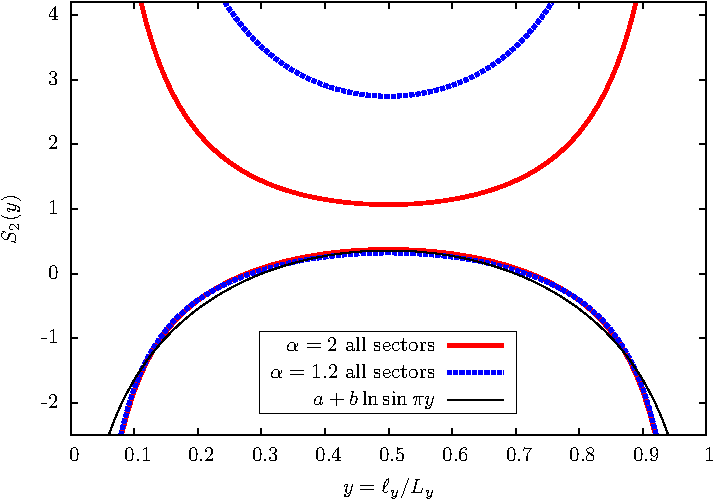
\includegraphics[width=8cm]{./figures/SUN_CFT.pdf}
 \end{center}
\caption{CFT prediction for the universal shape of $S_2$, as a function of $y=\ell_y/L_y$. Red solid lines correspond to the dimer RVB state with $\alpha=2$, while the blue dashed lines are the $SU(2)$ RVB case, with $\alpha= 1.2$.}
\label{fig:SUN_CFT}
\end{figure}
As is apparent from fig.~\ref{fig:SUN_CFT}, the curve for the even branch is essentially independent of the $\alpha$ over a large range. The shape of the odd curve only weakly depends on $\alpha$, but the curve does appreciably shift in this range.

Unfortunately, we do not know how to derive these results as we did for the dimers. The mapping of Ref.~\cite{Shannonee} to a classical R\'enyi-Shannon entropy is not valid for the $SU(N)$ RVB states: because of the non-orthogonality of different valence-bond configurations, the Schmidt decomposition of the RVB state is much more complicated.  Moreover, a naive extension of the result of \cite{Stephan2011} would then yield a critical value $ n_c=\alpha/2\simeq 0.6$  for $SU(2)$. This would imply an even-odd effect even for the von Neumann entropy, in violation with strong subadditivity\cite{Strongsubadditivity}. The formula $n_c=d_{\rm min }^2/(2\kappa)=d_{\rm min}^2\alpha/2$ therefore cannot hold in general for model which cannot be mapped onto a classical R\'enyi-Shannon entropy\footnote{The fact that it does apply to quantum six vertex states \emph{does not} contradict strong subadditivity, because in this case $d_{\rm min}=2$ and since $\alpha \geq 1$, we have $n_c\geq 1$. Notice that naively applying $n_c=d_{\rm min}^2 \alpha/2$ to an RK wave function built out of interacting dimers\cite{Alet_dimers1,Alet_dimers2} would also, just as $SU(N)$ RVB, violate strongsubadditivity.}.

Thus while we cannot make a definitive conclusion, our results provide qualitative evidence for Eq.~(\ref{eq:shape_general}) applying to the $SU(2)$ RVB state. They also support the convention of \cite{Ju2012} that the subleading piece of the two-cylinder Renyi entropy is universal.


% Even if such a mapping were still to hold in a renormalization group sense, exact diagonalization results on small system sizes clearly show that the biggest eigenvalue of the reduced density matrix is non degenerate, and therefore $d_{\rm min}=1$. This observation is also supported by the mapping to classical interacting dimers\cite{Damle}.


The same picture still seems to hold for the $SU(N)$ RVB state. We plot $S_2$ data for $L=16$ and $SU(2,3,4)$ is shown in Fig.~\ref{fig:SUN_shape}. As can be seen, the error bars get bigger and bigger for larger $N$, but we still observe a clear even-odd effect. This strongly suggest that we are still in a locked phase, and that Eq.~(\ref{eq:cft_prediction_gen}) applies in the thermodynamic limit. 
\begin{figure}[ht]
 \begin{center}
  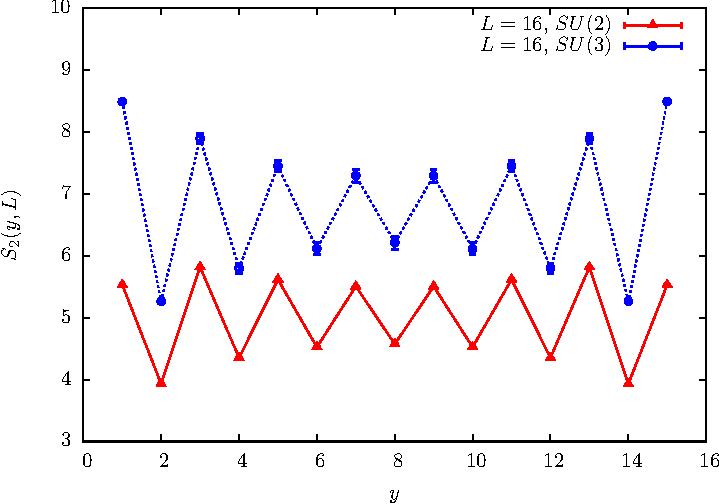
\includegraphics[width=10cm]{./figures/SUN_shape.pdf}
 \end{center}
\caption{Numerical data for the second R\'enyi entropy $S_2$ in the $SU(2,3,4)$ case. As can be seen, even on relatively small system sizes the numerical data is not totally converged. }
\label{fig:SUN_shape}
\end{figure}


>>> Maybe we should kill this bit, it isn't very convincing !!!
Extracting an accurate exponent $\alpha_N$ from the $S_2$ data is difficult, due to the combined finite-size effects and statistical errors. The most accurate way we found is to look at the even-odd difference for $y=1/2$. On the lattice it is defined as $\delta_n(L_x,L_y)=\left|S_n(L_y/2+1)-S_n(L_y/2)\right|$ for even $L_y$. This difference should go to a positive constant in the thermodynamic limit. From Eq.~(\ref{eq:cft_prediction_gen}) we predict
\begin{equation}\label{eq:even_odd}
 \delta_n(\tau,\alpha)=\frac{2n}{1-n}\ln \left(\frac{\theta_4(\alpha\tau/2)}{\theta_3(\alpha \tau/2)}\right)
\end{equation}
This allows in principle to determine the critical exponent from the entanglement data. Such an analysis is performed for quantum dimers as well as the $SU(2)$ RVB in Fig.~\ref{fig:evenodd}. As can be seen, finite-size effect again turn out to be very strong, even for quantum dimers. We observe the same kind of sublinear scaling for this quantity on small system sizes\cite{Ju2012}. However, as the $S_\infty$ data for quantum dimer can be rigorously shown to converge, it is reasonable to expect that the same happens for $S_2$.
\begin{figure}[ht]
\begin{center}
 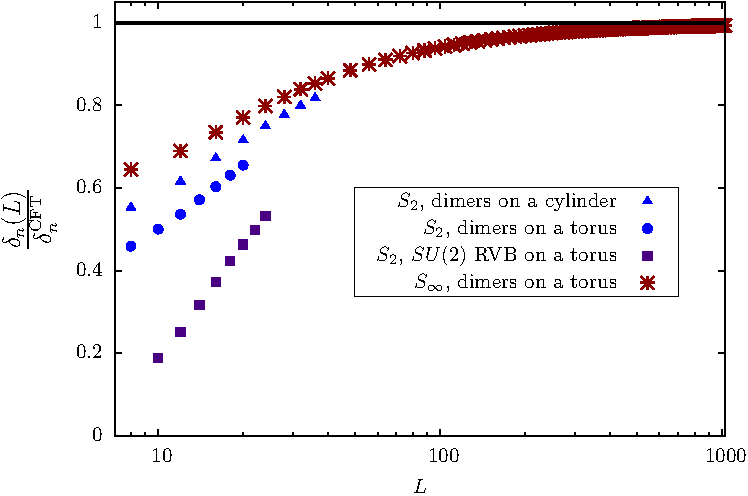
\includegraphics[width=8.1cm]{./figures/evenodd.pdf}
 %\hfill
 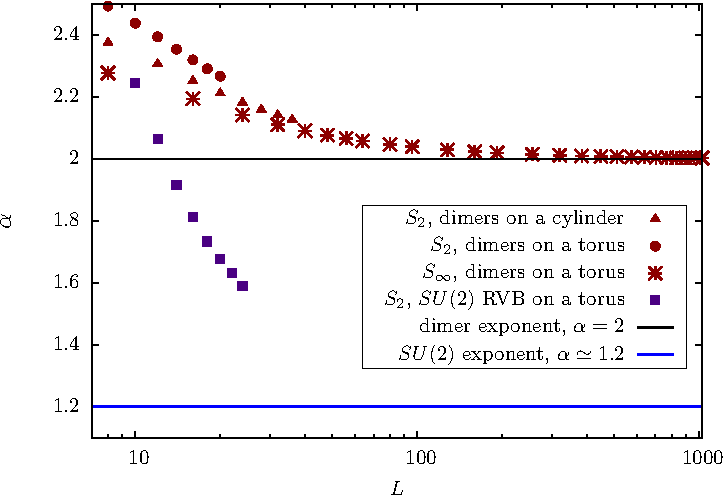
\includegraphics[width=8.1cm]{./figures/evenodd_alpha.pdf}
 \end{center}
 \caption{Even odd difference $\delta_n(L_x,L_y)=|S_n(L_x/2)-S_n(L_x/2-1)|$. \emph{Left Panel:} Convergence of $\delta_n(L)$ to the expected value from Eq.~(\ref{eq:even_odd}). \emph{Right Panel:} Finite-size extraction of $\alpha$ by solving $\delta_n(L_x,L_y)$ to Eq.~(\ref{eq:even_odd}). For quantum dimers as well as $SU(2)$, we observe an apparent sublinear scaling on small system sizes, which can be shown to go away for quantum dimers $S_\infty$.}
 \label{fig:evenodd}
\end{figure}

\section{Conclusion}

We have seen in the previous section (\ref{sec:rvb_entanglement}) that our main result seems to describe well, at least at the qualitative level, the entanglement data for $SU(2)$. There are two main reasons why such a result is non trivial

Resolving this issue is certainly an interesting question for further studies. It would also certainly be useful to change $d_{\rm min}$ by studying the RVB wave function on other bipartite lattices. For example on the hexagonal lattice $d_{\rm min}=3$ (and therefore $n_c=3^2=9$) for dimers, and $S_2$ for RVB would likely lie in the replicated phase, not subject to the even-odd effect. 


\label{sec:conclusion}
\textcolor{blue}{
\begin{itemize}
 \item Entanglement in finite $d>1$ critical systems. 
 \item Simple result for the shape dependence, as a ratio of known partition functions, not $\ln \sin$.
 \item Get a better understanding: change the lattice, Schmidt decomposition, \ldots.
 \item Extension to other RK points described by another CFT, generalizing\cite{Stephan2010,Zaletel}
 \item Hope this can help attack more complicated Quantum critical points.
\end{itemize}
}

\begin{itemize}
\item 
 From the perspective of the quantum dimer model, the R\'enyi entanglement entropy can be rewritten as a simple fidelity\cite{Bipartite_fidelity}:
 \begin{equation}\label{eq:lbf}
  S_{n>n_c}\sim \frac{n}{1-n} \ln \left|\langle A\cup B|A\otimes B\rangle\right|^2,
 \end{equation}
where $|A\cup B\rangle$ is the ground-state wave function of the whole system. $|A\otimes B\rangle$ is the ground-state wave function where all interactions between $A$ and $B$ have been switched off, a tensor product of the two ground-state wave functions in $A$ and $B$. Furthermore, Eq.~(\ref{eq:lbf}) even becomes exact on the lattice when $n\to \infty$.
 \item The universal shape we obtain bears strong resemblance to the numerical results of Ref.~\cite{Ju2012}, strengthening a posteriori the author's claim at universality.  
  \end{itemize}


\paragraph{Acknowledgments}
 We would like to thank Matthew Hastings for early collaboration on this project. We also thank Ann Kallin, Eduardo Fradkin, Gr\'egoire Misguich, Vincent Pasquier and \ldots for stimulating discussions. Grants acknowledgment. 
 \appendix
 \clearpage

\section[\;\;\;\;\;\;\;\;\;\;\;\;\;\;R\'enyi-Shannon entropy on the torus]{R\'enyi-Shannon entropy on the torus}
\label{sec:lgv}
>>> The definition of the fermions needs a little more explanation???
% Sites closest to the boundary are called ``boundary sites''.
%We attach an $\uparrow$ (resp. $\downarrow$) virtual spin to a boundary site occupied by a dimer in $B$ (resp. $A$) and represent it by a black (resp. white) filled circle. Each boundary configuration has probability $p_{\sigma,\mu}$. \emph{Left}: Example of dimer configuration compatible with $|\sigma\rangle=|\!\uparrow\uparrow\downarrow\downarrow\uparrow\uparrow\uparrow\downarrow\rangle$ and $|\mu\rangle=|\!\downarrow\uparrow\downarrow\uparrow\downarrow\downarrow\uparrow\downarrow\rangle$. \emph{Right}: Example of dimer configuration compatible with the most likely boundary configuration $|\sigma\rangle=|\!\uparrow\uparrow\uparrow\uparrow\uparrow\uparrow
%\uparrow\uparrow\rangle$ and $|\mu\rangle=|\!\downarrow\downarrow\downarrow
%\downarrow\downarrow\downarrow\downarrow\downarrow\rangle$, where no dimers are crossing the boundary.

We wish to compute the following classical entropy
\begin{equation}
 S_n=\frac{1}{1-n} \ln \left(\sum_{\sigma,\mu} [p_{\sigma,\mu}]^n\right), 
\end{equation}
for any real $n$. The probabilities $p_{\sigma,\mu}$ we are interested in are given by a ratio of partition functions, which can handily be expressed using a transfer matrix
\begin{equation}\label{eq:tm}
 p_{\sigma,\mu}=\frac{Z_{\sigma,\mu}^A Z_{\mu,\sigma}^B}{Z}=\frac{\langle  \sigma|T^{\,\ell_y}|\mu\rangle\langle \mu|T^{\,L_y-\ell_y}|\sigma\rangle}{{\rm Tr}\; T^{L_y}}
\end{equation}
$T$ is the transfer matrix of the dimer model, and acts on the vector space generated by dimer occupancies on vertical edges along a horizontal line: $\langle a|T|b\rangle=1$ if configuration $|a\rangle$ and $|b\rangle$ are compatible, $0$ otherwise. The denominator is calculated in \ref{sec:dimers_exact}. Each factor on the numerator of Eq.~(\ref{eq:tm}) can be evaluated by a mapping onto free fermions\cite{Lieb1967,Alet_dimers2,Shannonee}, as explained in Fig.~\ref{fig:freefermions}.  
\begin{figure}[ht]
\begin{center}
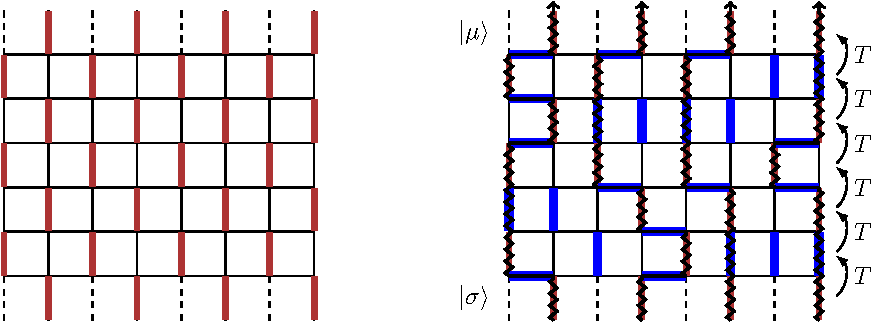
\includegraphics{./figures/free_fermions.pdf}
  \end{center}
  \caption{Illustration of the mapping onto free fermions. \emph{Left:} reference configuration with staggered dimers. \emph{Right:} transition graph generated by superimposing the reference configuration on the actual dimer configuration (in blue). This generates a collection of non-intersecting lattice paths, which can handily be expressed in terms of fermions. }
  \label{fig:freefermions}
  \end{figure}
A fermion is defined as an even vertical link occupied by a dimer, or an odd vertical empty link. $|\sigma\rangle$ and $|\mu\rangle$ can be rewritten in the antisymmetric fermionic basis
\begin{eqnarray}
|\sigma \rangle&=&|x_1,x_2,\ldots,x_N\rangle=c_{x_1}^\dag c_{x_2}^\dag \ldots c_{x_N}^\dag |0\rangle \\
|\mu \rangle&=&|y_1,y_2,\ldots,y_N\rangle=c_{y_1}^\dag c_{y_2}^\dag \ldots c_{y_N}^\dag |0\rangle
\end{eqnarray}
where the $x_i$ and $y_j$ label the ordered positions of the fermions. Introducing of shift of $+1$ lattice spacing from one row to the other, it is easy to check from Fig.~\ref{fig:freefermions} that the transfer matrix satisfies
\begin{eqnarray}
T|0\rangle&=&|0\rangle\\
T c_{2j}^\dag T^{-1}&=&c_{2j}^\dag+c_{2j+1}^\dag +c_{2j+2}^\dag\\
T c_{2j+1}^\dag T^{-1}&=&c_{2j+2}^\dag
\end{eqnarray}
Periodic boundary condition implies $c_{L_x}^\dag=(-1)^{N+1}c_0^\dag$. Writing this in matrix form using Einstein's summation convention
\begin{equation}
 T c_i^\dag T^{-1}=M_{ij} c_j^\dag,
\end{equation}
we successively get
\begin{equation}
 T^\ell c_i^\dag T^{-\ell}=\left(M^\ell\right)_{ij} c_j^\dag
\end{equation}
and 
\begin{eqnarray}
\langle \sigma |T^\ell |\mu\rangle&=&\langle 0|c_{x_1} c_{x_2} \ldots c_{x_N} T^{\ell} c_{y_1}^\dag c_{y_2}^\dag \ldots c_{y_N}^\dag |0\rangle \\ 
&=&\langle 0|c_{x_1} c_{x_2} \ldots c_{x_N} (M^\ell)_{y_1 z_1}c_{z_1}^\dag (M^\ell)_{y_2 z_2}c_{z_2}^\dag \ldots (M^\ell)_{y_N z_N}c_{z_N}^\dag|0\rangle
\end{eqnarray}
By applying the Wick's theorem and using $\langle 0|c_x c_y^\dag|0\rangle=\delta_{xy}$, we finally get
\begin{equation}
 \langle \sigma |T^\ell |\mu\rangle=\det_{1\leq i,j\leq N} \left[(M^\ell)_{x_i y_j}\right]
\end{equation}
This type of result is referred to as the Karlin-McGregor\cite{KarlinMcGregor} or Lindstr\"om-Gessel-Viennot\cite{Lindstrom1973,GesselViennot1989} lemna in the mathematical litterature. In the end, Eq.~(\ref{eq:tm}) reduces to a product of two determinants, which may be computed numerically.
\section[\;\;\;\;\;\;\;\;\;\;\;\;\;\;CFT correlations and partition functions]{CFT correlations and partition functions}
\label{sec:CFT_Jacobi}
%\subsection[\;\;\;\;\;\;\;\;\;\;\;\;\;\;Dedekind-eta and Jacobi-Theta functions]{Dedekind-eta and Jacobi-Theta functions}
%\label{sec:functions}
For a given modulus $\tau$, we introduce the squared nome:
\begin{equation}
 q=e^{2i\pi \tau}
\end{equation}
The Dedekind eta function is defined as 
\begin{equation}\label{eq:eta_def}
 \eta(\tau)=q^{1/ 24}\prod_{k=1}^{\infty}\left(1-q^k\right),
\end{equation}
and the four Jacobi Theta functions are given by
\begin{eqnarray}\label{eq:theta1_def}
 \theta_1(z|\tau)&=&\sum_{n \in \mathbb{Z}}(-1)^{n-1/2}q^{\frac{1}{2}(n+1/2)^2}e^{(2n+1)iz}\\
 &=&2\eta(\tau)q^{1/6} \sin z\prod_{n=1}^{\infty} \left[1-2 \cos(2z) q^{n}+q^{2n}\right]
\end{eqnarray}
\begin{eqnarray}\label{eq:theta2_def}
 \theta_2(z|\tau)&=&\sum_{n \in \mathbb{Z}}q^{\frac{1}{2}(n+1/2)^2}e^{(2n+1)iz}\\
 &=&2\eta(\tau)q^{1/6} \cos z\prod_{n=1}^{\infty} \left[1+2 \cos(2z) q^{n}+q^{2n}\right]
\end{eqnarray}
\begin{eqnarray}\label{eq:theta3_def}
 \theta_3(z|\tau)&=&\sum_{n \in \mathbb{Z}}q^{\frac{1}{2}n^2}e^{2niz}\\
 &=&\eta(\tau)q^{-1/12}\prod_{n=1}^{\infty} \left[1+2 \cos(2z) q^{n-1/2}+q^{2n-1}\right]
\end{eqnarray}
\begin{eqnarray}\label{eq:theta4_def}
 \theta_4(z|\tau)&=&\sum_{n \in \mathbb{Z}}(-1)^{n}q^{\frac{1}{2}n^2}e^{2niz}\\
 &=&\eta(\tau)q^{-1/12}\prod_{n=1}^{\infty} \left[1-2 \cos(2z) q^{n-1/2}+q^{2n-1}\right]
\end{eqnarray}
To simplify the notations a bit, we also set
\begin{equation}\label{eq:thetas}
 \theta_\nu(\tau)=\theta_\nu (0|\tau)\quad,\quad \nu=1,2,3,4
\end{equation}

These functions obey the following nice ``modular'' transformation properties
\begin{eqnarray}
 \theta_1(\tau)&=&-i (-i \tau )^{-1/2}\,\theta_1(-1/\tau)\\
 \theta_2(\tau)&=&(-i \tau )^{-1/2}\,\theta_4(-1/\tau)\\\label{eq:modtheta3}
 \theta_3(\tau)&=&(-i \tau )^{-1/2}\,\theta_3(-1/\tau)\\\label{eq:modtheta4}
 \theta_4(\tau)&=&(-i \tau )^{-1/2}\,\theta_2(-1/\tau)\\\label{eq:modeta}
 \eta(\tau)&=&(-i \tau )^{-1/2}\,\eta(-1/\tau)
\end{eqnarray}
%\subsection[\;\;\;\;\;\;\;\;\;\;\;\;\;\;Partition functions in various geometries for the free boson]{Partition functions in various geometries for the free boson}
%\label{sec:free_boson}
%Here $\tau=iL_y/L_x$, for a cylinder of circumference $L_x$ and height $L_y$. The calculation of partition function in torus and cylinder with various boundary condition is standard, see for example\cite{EggertAffleck,FSW,BigYellowBook}. We list some of them below.
%\begin{itemize}
% \item Cylinder with Dirichlet boundary condition at both ends (even case in the text). 
% \begin{equation}\label{eq:cylinder_dd}
% \mathcal{Z}_{\rm cyl}^{DD}=g_{D}^2 \,\frac{\theta_3(\alpha \tau)}{\eta(2\tau)}
%\end{equation}
%\item Cylinder with the shifted Dirichlet boundary condition discussed in the text (winding quantized with half-integer values, corresponding to the odd case):
%\begin{equation}\label{eq:cylinder_ddprime}
% \mathcal{Z}_{\rm cyl}^{DD^\prime}=g_{D}^2 \,\frac{\theta_4(\alpha \tau)}{\eta(2\tau)}
%\end{equation}
%\item Cylinder with Neuman at one end, and Dirichlet at the other:
%\begin{equation}
% {\cal Z}_{\rm cyl}^{ND}=g_N g_D \, \frac{\theta_4(4\tau)}{\eta(2\tau)}
%\end{equation}
%\item Torus partition function
%\begin{equation}
% {\cal Z}_{\rm torus}=\frac{\theta_3(\alpha \tau)\theta_3(\tau /\alpha)}{\eta(\tau)^2}
%\end{equation}
%\end{itemize}
%$g_D$ and $g_N$ are the universal Affleck-Ludwig\cite{AffleckAndLudwig,FSW} g-factors, corresponding to the Dirichlet and Neuman boundary condition respectively.
%\begin{eqnarray}
% g_D&=& (\alpha/2)^{1/4}\\
% g_N&=& (2\alpha)^{-1/4}
%\end{eqnarray}


\section[\;\;\;\;\;\;\;\;\;\;\;\;\;\;CFT partition functions from the lattice dimer model]{Derivation of CFT partition function from the lattice dimer model}
\label{sec:dimers_exact}
 \subsection[\;\;\;\;\;\;\;\;\;\;\;\;\;\; Torus]{Torus}
The goal of this section is to recover the CFT partition function on the torus, using the exact solution for dimers in terms of transfer matrix, and keeping track of the winding numbers $W_x$ and $W_y$. To do that we need to solve a slightly more complicated problem than that in \ref{sec:lgv}, introducing a fugacity $b$ (resp. $b^{-1}$) for horizontal dimers whose left site belongs to the even (resp. odd) sublattice. We will also suppose $L_x$ and $L_y$ to be even. With this at hand the transfer matrix now satisfies
\begin{eqnarray}
T|0\rangle&=&|0\rangle\\
T c_{2j}^\dag T^{-1}&=&b \,c_{2j}^\dag+c_{2j+1}^\dag +b^{-1}c_{2j+2}^\dag\\
T c_{2j+1}^\dag T^{-1}&=&c_{2j+2}^\dag
\end{eqnarray}
The $b$'s provide information about $W_x$, while the number of fermions does that for $W_y$. 
Defining as before $T c_i^\dag T^{-1}=M_{ij} c_j^\dag$, diagonalizing $T$ amounts to diagonalizing $M$, which can be done in Fourier space, carefully taking into account the boundary condition on fermions
\begin{equation}
 c_{L_x}^\dag=(-1)^{\hat{N}+1}c_0^\dag\quad,\quad \hat{N}=\sum_{j=1}^{L_x} c^\dag_j c_j
\end{equation}
We write the number of dimer coverings in the $(W_x,W_y)$ sector as $Z_{W_x,W_y}$. Setting $b=e^{-\pi u_x/L_x}$, the winding generating function is given by
\begin{eqnarray}
 Z(u_x,u_y)&=&\sum_{W_x,W_y} Z_{W_x,W_y}e^{-\pi (W_x u_x+W_y u_y)}\\\label{eq:Z_tm}
 &=&{\rm Tr}\left[\displaystyle{e^{-\pi u_y(\hat{N}-L_x/2)/2}T^{L_y}}\right]
\end{eqnarray}
If we now denote by $d_k^\dag$ the set of fermionic operators that diagonalize the one-particle transfer matrix
\begin{equation}
 T d_k^\dag T^{-1}=\lambda_k d_k^\dag,
\end{equation}
the $\lambda_k$ are then the eigenvalues of $M$. Using this, the transfer matrix can be expressed as
\begin{equation}
 T=\prod_k \left(1+[\lambda_k -1]d_k^\dag d_k \right)
\end{equation}
Plugging this expression in Eq.~(\ref{eq:Z_tm}) we get\footnote{One can check easily that expanding simultaneously the first two product in Eq.~(\ref{eq:dimers_torus}) generates all the eigenvalues of the transfer matrix in the even fermion sector. The same goes for the last two products and the odd-fermions sector. }
\begin{eqnarray}\nonumber
 Z(u_x,u_y)&=&\prod_{k\in \Omega_{1}}\left[e^{\pi x /2}+e^{-\pi x/2}\lambda_k^{L_y}\right]+\prod_{k\in \Omega_{1}}\left[e^{\pi x/2}-e^{-\pi x/2}\lambda_k^{L_y}\right]\\\label{eq:dimers_torus}
 &+&\prod_{k\in \Omega_{0}}\left[e^{\pi x /2}+e^{-\pi x/2}\lambda_k^{L_y}\right]-\prod_{k\in \Omega_{0}}\left[e^{\pi x /2}-e^{-\pi x/2}\lambda_k^{L_y}\right]
\end{eqnarray}
with
\begin{eqnarray}
 \lambda_k&=&\cos k +\sqrt{1+\cos^2 k}\\
\Omega_{\nu}&=&\left\{\frac{(2m+\nu+i u_y) \pi}{L_x}\quad,\quad m=-L_x/2,\ldots,L_x/2-1\right\} 
\end{eqnarray}
Of course, $Z(u_x=0,u_y=0)$ reduces to the well known torus partition function obtained by Kasteleyn and Fisher. 
\paragraph{}We now wish to extract the universal CFT partition function $\mathcal{Z}$, i.e the constant term in the asymptotic expansion of $Z$:
\begin{equation}
 Z(u_x,u_y)\sim A^{L_x L_y} B^{L_x} C^{L_y}\mathcal{Z}(u_x,u_y)
\end{equation}
A possible way to do so would be to combine Euler-Maclaurin expansions and majoration techniques, as has already been done for the honeycomb lattice\cite{Boutillier}. Here we obtain $\mathcal{Z}$ in a more heuristic (and non rigorous) manner, noticing that universal properties have to come from low energy excitation near the Fermi momenta $k_F=\pm \pi/2$. Linearizing $\ln(\lambda_k)$ around the two $k_F$ and extending the products in \ref{eq:dimers_torus} over all integers, allows to go get after a long calculation, very similar to that in \cite{Boutillier}:
\begin{equation}
 \mathcal{Z}(u_x,u_y)=\frac{\displaystyle{\theta_3(i\pi u_x/2|\tilde{\tau}/2)\,\theta_3(i\pi u_y/2|\tau/2)}}{\displaystyle{(2 \Im{\rm m}\, \tau)^{1/2}\,\eta(\tau)^2}}
\end{equation}
where $\tau=i L_y/L_x$ and $\tilde{\tau}=-1/\tau=iL_x/L_y$. 
\subsection[\;\;\;\;\;\;\;\;\;\;\;\;\;\; Cylinder]{Cylinder}
The cylinder geometry is slightly simpler than its torus counterpart, because only the windings along $y$ are allowed. To still express the partition function as a trace, we look at the transfer matrix $\tilde{T}$ acting on the configuration of rows of length $L_y$ with \emph{open} boundary conditions. This way, the number of fermions keeps track of the winding number $W_y$. The winding generating function can be expressed, after some algebra, as
\begin{eqnarray}
 Z(u_y)&=&e^{-\pi (L_y/2)u_y}\prod_{m=1}^{L_y} \left(1+e^{\pi u_y}\mu_m^{L_x}\right)\\
 \mu_m&=&\cos \left(\frac{m \pi}{L_y+1}\right)+\sqrt{1+\cos^2\left(\frac{m \pi}{L_y+1}\right)}
\end{eqnarray}
Here the Fermi momentum is $k_F=\pi/2$, and the CFT partition function can be accessed using the linearization trick. We, however have to distinguish between the even and odd $L_y$ cases.
\paragraph{Even case}
It is most convenient to rewrite $Z$ as
\begin{equation}
Z(u_y)=\prod_{m=1}^{L_y/2} \lambda_m^{L_x}\times \left[\prod_{m=1}^{L_y/2} 1+2\cosh (\pi u_y)\mu_m^{-L_x}+\mu_m^{-2L_x}\right] 
\end{equation}
Combining the Euler-Maclaurin formula on the first product, and using the linearization procedure around $m=L_y/2$, we get
\begin{equation}
 \mathcal{Z}= e^{\frac{\pi L_x}{24 L_y}}\prod_{p=1}^{\infty}\left[1+2 \cosh (\pi u_y)e^{-\frac{\pi L_x}{L_y}(p-1/2)}+e^{-2\frac{\pi L_x}{L_y}(p-1/2)}\right]
\end{equation}
which gives, using the infinite product representation of the Jacobi Theta function,
\begin{equation}
 \mathcal{Z}=\frac{\theta_3(i \pi u_y/2|\tilde{\tau}/2)}{\eta(\tilde{\tau}/2)}
\end{equation}
We recover the CFT result (\ref{eq:cylinder_dd}), upon setting $u_y=0$ and performing a modular transformation. 
\paragraph{Odd case}
We use the same method, but care must be taken because of the presence of a zero-mode for $m=(L_y+1)/2$ We have
\begin{equation}
Z(u_y)=2\cosh(\pi u_y/2)\prod_{m=1}^{(L_y-1)/2} \lambda_m^{L_x}\times \left[\prod_{m=1}^{(L_y-1)/2} 1+2\cosh (\pi u_y)\mu_m^{L_x}+\mu_m^{2L_x}\right] 
\end{equation}
which yields after linearization
\begin{equation}
 \mathcal{Z}= 2 e^{-\frac{\pi L_x}{12 L_y}}\cosh(\pi u_y/2)\prod_{p=1}^{\infty}\left[1+2 \cosh (\pi u_y)e^{-\frac{\pi L_x}{L_y}p}+e^{-2\frac{\pi L_x}{L_y}p}\right]
\end{equation}
In the end we obtain:
\begin{equation}
 \mathcal{Z}=\frac{\theta_2(i \pi u_y/2|\tilde{\tau}/2)}{\eta(\tilde{\tau}/2)}
\end{equation}
and once again recover the CFT result (\ref{eq:cylinder_ddprime}) after setting $u_y=0$ and modular transformation. 
\subsection[\;\;\;\;\;\;\;\;\;\;\;\;\;\; Zero-winding sectors]{Zero-winding sectors}
With the winding generating function at hand, the calculation of $s_n(y,\tau)$ in the $W=(0,0)$ winding sector becomes straightforward. For example we have (recall $\tau=iL_y/L_x$ and $\tilde{\tau}=-1/\tau$)
\begin{eqnarray}\label{eq:nullwinding1}
\underbrace{\mathcal{Z}_{\rm cyl}^{DD^\prime}(y\tau)\mathcal{Z}_{\rm cyl}^{DD^\prime}((1-y)\tau)}_{W=(0,0)}&=&\frac{1}{\eta(\frac{\tilde{\tau}}{2y})\eta(\frac{\tilde{\tau}}{2(1-y)})} 
\underbrace{\theta_2\left(\frac{i \pi u_y}{2}\right.\left|\frac{\tilde{\tau}}{2y}\right)\theta_2\left(\frac{i \pi u_y}{2}\right.\left|\frac{\tilde{\tau}}{2(1-y)}\right)}_{W=(0,0)}\\\label{eq:nullwinding2}
&=&\frac{\theta_2\Big(0\left|\frac{\tilde{\tau}}{2y(1-y)}\right)}{\eta(\frac{\tilde{\tau}}{2y})\eta(\frac{\tilde{\tau}}{2(1-y)})}
\end{eqnarray}
Eq.~(\ref{eq:nullwinding2}) follows from Eq.~(\ref{eq:nullwinding1}) by selecting the term in $(u_y)^0$ in the product of theta functions. This allows to recover Eq.~(\ref{eq:cft_w0_gen}) and Eq.~(\ref{eq:cft_w0_gen2}) after once again a modular transformation. 
 \section*{References}
\bibliography{rvb4_bib.bib}{}
\bibliographystyle{unsrt}


\end{document}



% utilized in \cite{Ju2012}, for RK-type states. The torus has dimensions $L_x$ and $L_y$, and is cut i%nto two cylinders of dimensions $L_x \times \ell_y$ and $ L_x \times (L_y-\ell_y)$
% \begin{figure}[ht]
%  \begin{center}
%   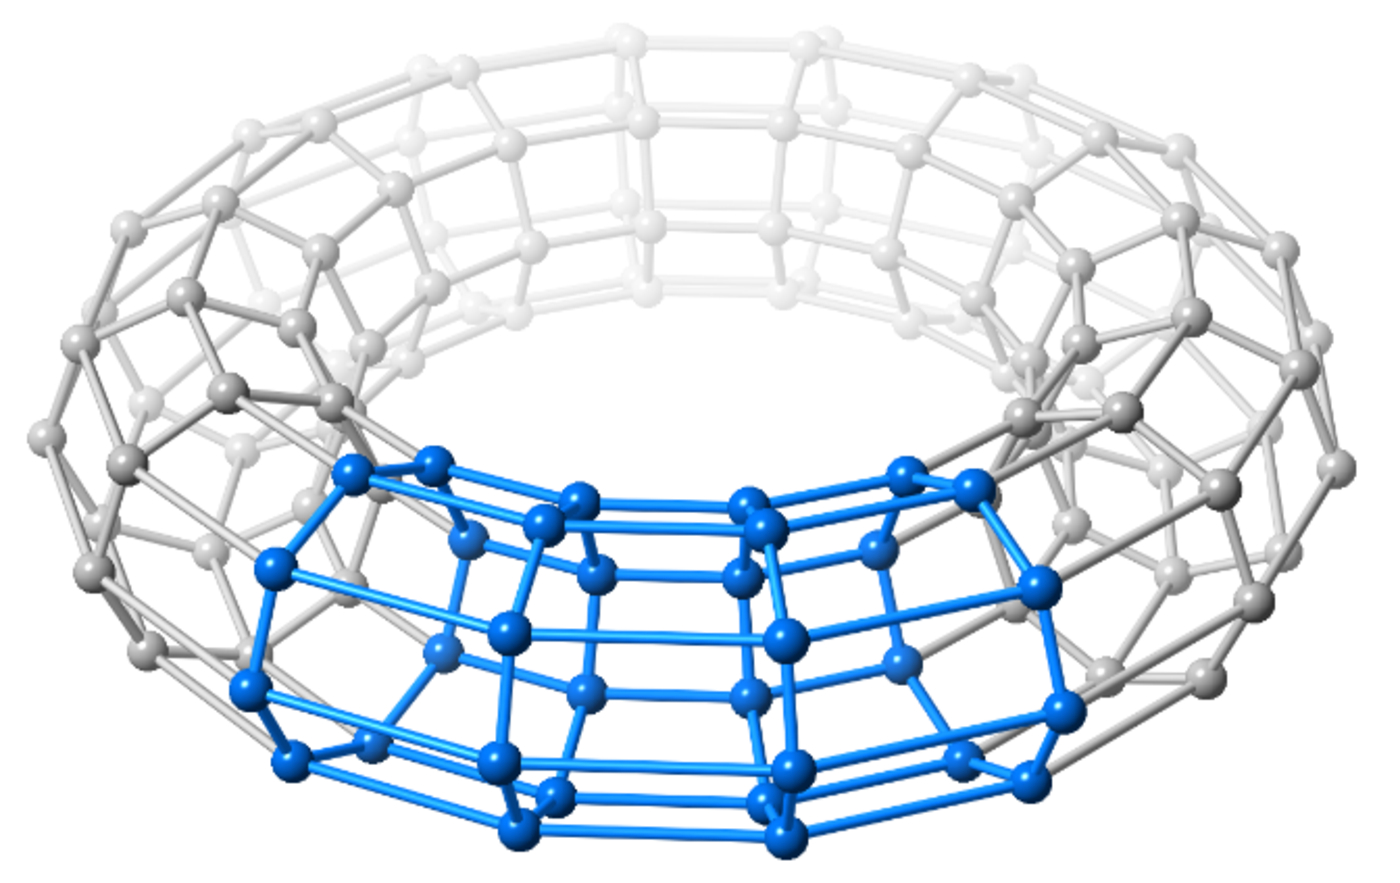
\includegraphics[width=7cm,angle=-90]{./figures/16x8b.pdf}
%   \end{center}
%   \caption{Torus geometry studied in this paper, with $L_x=8$ and $L_y=16$. We mainly focus on entanglement aspects. The system is cut into two parts $A$ and $B$. Here subsystem $A$ is a cylinder of height $\ell_y=4$, and is drawn in bold blue. Subsystem $B$ is a cylinder of height $L_y-\ell_y=12$. We are particularly interested in the dependence of entanglement on the shape $\ell_y/L_y$, $L_x/L_y$ of the torus.}
% \label{fig:torus}
%  \end{figure}
% Physical results are expected to only depend on the two possible dimensionless ratios $L_y/L_x$ and $\ell_y/L_y$. The first is encoded in the modulus $\tau$ of the torus:
% \begin{equation}
%  \tau=i\frac{L_y}{L_x}.
% \end{equation}
% The imaginary number is there for later convenience, as it allows to make contact with standard results from conformal field theory. Most of the numerical studies will be performed for the most natural $L_y=L_x$ case, but we expect our results to be valid for any aspect ratio. We call the other ratio
% \begin{equation}
%  y=\frac{\ell_y}{L_y}
% \end{equation}
% the ``subsystem ratio''. It plays the same role as the $x/L$ in 1d. We are interested in the scaling behavior of the entropy with $L$, while keeping both ratios $y$ and $\tau$ finite. 
% \paragraph{}
%  It is well known that the R\'enyi entanglement entropy of such quantum systems exhibits an area law\cite{ALreview}:
%  \begin{equation}
%  S_n(L,y,\tau)= a_{n} L+s_{n}(y,\tau)+\mathcal{O}(1/L)
% \end{equation}
% Since the boundary between $A$ and $B$ is smooth and assuming a Coulomb gas description, we expect no subleading logarithmic corrections\cite{Hsu2009}. The first subleading term should be a universal constant $s_n(y,\tau)$, which depends only on the two aspect ratios for a given universality class. At this stage it is important to notice that although $a_n$ is non-universal -- and therefore depends on the specifics of the lattice model -- this area law term should \emph{not} depend on the two aspect ratios. This simple fact has an important practical consequence: one can read off the $y$ (or $\tau$) dependence of $s_n(y,\tau)$ by just looking at the numerical data $S_n(L,y,\tau)$ for sufficiently large $L$. We will use this method\cite{Ju2012} throughout the paper, therefore sidestepping any  (possibly difficult in practice) fitting procedure.    



